% Relatório técnico no padrão ABNT (abnTeX2) - gerado a partir do modelo da skill relatorio-abnt

\documentclass[12pt, oneside, a4paper, sumario=tradicional, chapter=TITLE, brazilian]{abntex2}

\usepackage{fontspec}
\setmainfont{LiberationSans}[Path=/usr/share/fonts/truetype/liberation/, Extension=.ttf, UprightFont=*-Regular, BoldFont=*-Bold, ItalicFont=*-Italic, BoldItalicFont=*-BoldItalic]  % métrica idêntica à Arial
\setmonofont{LiberationMono}[Path=/usr/share/fonts/truetype/liberation/, Extension=.ttf, UprightFont=*-Regular, BoldFont=*-Bold, ItalicFont=*-Italic, BoldItalicFont=*-BoldItalic, Scale=0.95]
\usepackage{indentfirst}
\usepackage[table]{xcolor}
\usepackage{graphicx}
\usepackage{microtype}
\usepackage{amsmath, amssymb}
\usepackage{array}
\usepackage{float}
\usepackage{pdflscape}
\usepackage{fvextra}
\usepackage{enumitem}
\usepackage{url}
\usepackage{chngcntr}
\usepackage{ragged2e}
\usepackage[alf]{abntex2cite}

\counterwithout{figure}{chapter}
\counterwithout{table}{chapter}
\counterwithout{equation}{chapter}

\setlrmarginsandblock{3cm}{2cm}{*}
\setulmarginsandblock{3cm}{2cm}{*}
\checkandfixthelayout
\setlength{\parindent}{1.25cm}
\setlength{\parskip}{0.0cm}
\OnehalfSpacing
\setlength{\abovecaptionskip}{4pt}
\renewcommand{\ABNTEXchapterfont}{\bfseries}
\renewcommand{\ABNTEXchapterfontsize}{\normalsize}
\renewcommand{\ABNTEXsectionfont}{\bfseries}
\renewcommand{\ABNTEXsectionfontsize}{\normalsize}
\renewcommand{\ABNTEXsubsectionfont}{\bfseries}
\renewcommand{\ABNTEXsubsectionfontsize}{\normalsize}
\setlength{\afterchapskip}{18pt}
\setlength{\beforechapskip}{0pt}
\captionnamefont{\small}
\captiontitlefont{\small}
\renewcommand{\arraystretch}{1.3}

\titulo{ENLACE DE DADOS CONFIÁVEL VIA RÁDIO DE 433 MHz ENTRE DUAS ESP32: Detecção de erros por CRC-8 e controle de erros por \textit{Selective Repeat} ARQ}
\autor{KAUAN SANTOS RONDON \\ LUIS FERNANDO AMORIM DA SILVA \\ VINÍCIUS CAMPOS ANDRADE SILVA}
\local{Cuiabá – MT}
\data{2026}
\instituicao{INSTITUTO FEDERAL DE EDUCAÇÃO, CIÊNCIA E TECNOLOGIA DE MATO GROSSO \\ CAMPUS CUIABÁ – CEL. OCTAYDE JORGE DA SILVA}
\tipotrabalho{Relatório técnico}
\orientador[Professor:]{Ruy de Oliveira}
\preambulo{Relatório técnico apresentado como requisito parcial de avaliação na disciplina Transmissão e Comunicação de Dados do curso de Bacharelado em Engenharia da Computação do Instituto Federal de Educação, Ciência e Tecnologia de Mato Grosso, Campus Cuiabá – Cel. Octayde Jorge da Silva.}

\hypersetup{hidelinks, pdftitle={Enlace de dados confiável via rádio de 433 MHz entre duas ESP32}, pdfauthor={Kauan Santos Rondon; Luis Fernando Amorim da Silva; Vinícius Campos Andrade Silva}, pdfsubject={Relatório técnico - Transmissão e Comunicação de Dados - IFMT}, pdfkeywords={RF 433 MHz; ESP32; CRC-8; Selective Repeat}}
\begin{document}
\selectlanguage{brazilian}
\frenchspacing

% ---------------- Capa com a logo do IFMT
\begin{capa}
  \centering
  
\includegraphics[width=7.5cm]{fig/logo_ifmt.png}\par\vspace{0.8cm}
  {\bfseries\ABNTEXchapterfont INSTITUTO FEDERAL DE EDUCAÇÃO, CIÊNCIA E TECNOLOGIA DE MATO GROSSO\par
   CAMPUS CUIABÁ – CEL. OCTAYDE JORGE DA SILVA\par}
  \vspace{0.2cm}{\normalfont BACHARELADO EM ENGENHARIA DA COMPUTAÇÃO\par}
  \vspace{2.2cm}
  {\bfseries KAUAN SANTOS RONDON \\ LUIS FERNANDO AMORIM DA SILVA \\ VINÍCIUS CAMPOS ANDRADE SILVA\par}
  \vfill
  {\bfseries\large ENLACE DE DADOS CONFIÁVEL VIA RÁDIO DE 433 MHz ENTRE DUAS ESP32\par}
  \vspace{0.4cm}
  {Detecção de erros por CRC-8 e controle de erros por \textit{Selective Repeat} ARQ\par}
  \vfill\vfill
  {\imprimirlocal\par \imprimirdata\par}
\end{capa}

\imprimirfolhaderosto*

\begin{resumo}
 \SingleSpacing
 Este relatório descreve o projeto, a implementação e a avaliação experimental de um enlace de dados unidirecional e confiável entre duas placas ESP32, com comunicação exclusivamente por módulos de rádio de 433 MHz (FS1000A e MX-RM-5V) e sem bibliotecas de rádio. A camada física foi construída sobre a UART da ESP32 a 1200 bit/s, com sinal invertido, preâmbulo de sincronização, delimitador 0x7E e codificação Manchester. Os dados trafegam em quadros com os campos FLAG, TYPE, SEQ, LEN, DATA e FCS, limitados a 21 bytes. A detecção de erros utiliza CRC-8 com polinômio gerador x⁸ + x² + x + 1, e o controle de erros utiliza \textit{Selective Repeat ARQ} com janela de até 8 quadros e confirmações com mapa de bits. O receptor exibe os textos recebidos em um LCD 16x2 e repassa as imagens ao computador. Em uma bateria de 36 ensaios, 33 mensagens foram entregues sem nenhum erro, incluindo seis imagens cujo resumo SHA-256 coincidiu com o do arquivo original, com distâncias de até 2 m e sob interferência real. Em validação posterior, com uma placa em cada computador, 19 de 21 mensagens foram entregues sem erro, com falhas apenas a 2 m, e uma imagem de 2866 bytes foi transferida íntegra a 1,8 m. O cálculo do CRC consumiu cerca de 8 µs por quadro, e a janela de 8 quadros reduziu em 56\% o tempo de entrega em relação ao \textit{Stop-and-Wait}. As três mensagens não entregues foram abandonadas pelo transmissor após 20 s sem confirmação, sem entrega de dado corrompido.

 \vspace{\onelineskip}
 \noindent\textbf{Palavras-chave}: RF 433 MHz; ESP32; CRC-8; Selective Repeat; controle de erros; enlace de dados.
\end{resumo}

\pdfbookmark[0]{\listfigurename}{lof}
\listoffigures*
\cleardoublepage
\pdfbookmark[0]{\listtablename}{lot}
\listoftables*
\cleardoublepage
\pdfbookmark[0]{\contentsname}{toc}
\tableofcontents*
\cleardoublepage

\textual
\pagestyle{simple}\aliaspagestyle{chapter}{simple}

\chapter{INTRODUÇÃO}
Canais de rádio de baixo custo, como os módulos OOK de 433 MHz, perdem e corrompem quadros com frequência, seja por atenuação, por reflexões no ambiente ou por interferência de outros equipamentos. Para que uma aplicação receba os dados sem erro sobre um meio desse tipo, a camada de enlace precisa executar duas funções: detectar os quadros corrompidos e recuperar os que se perderam (FOROUZAN, 2010; TANENBAUM; WETHERALL, 2011).

O projeto final da disciplina Transmissão e Comunicação de Dados propõe a implementação dessas funções em um enlace real entre duas placas ESP32, com comunicação exclusivamente por rádio e sem o uso de bibliotecas como a RadioHead (IFMT, 2026). A placa A atua como transmissora e a placa B como receptora; os dados seguem de A para B e as confirmações retornam de B para A. O receptor apresenta o texto recebido em um display LCD e o computador ligado a ele reconstrói as imagens recebidas.

O enunciado avalia o projeto pelo algoritmo de detecção de erros (soma de verificação ou CRC) e pelo algoritmo de controle de erros (\textit{Stop-and-Wait}, \textit{Go-Back-N} ou \textit{Selective Repeat}), além de critérios de aceitação: comunicação a mais de 1 m, funcionamento sob ruído, uso exclusivo do rádio e entrega dos dados em perfeito estado. Este trabalho adotou as opções de maior complexidade em ambos os algoritmos, CRC e \textit{Selective Repeat}.

\section{Objetivo geral}

Implementar e avaliar experimentalmente um enlace de dados confiável entre duas ESP32 por rádio de 433 MHz, capaz de transmitir texto e imagens pequenas sem erro a distâncias superiores a 1 m e em presença de ruído.

\section{Objetivos específicos}

\begin{enumerate}[label=\alph*),leftmargin=1.9cm,itemsep=2pt]
  \item montar o \textit{hardware} das duas placas, com um transmissor e um receptor de rádio em cada uma e o LCD na placa receptora;
  \item implementar a transmissão de rádio sem bibliotecas, com o quadro definido no enunciado;
  \item implementar a detecção de erros com CRC-8;
  \item implementar o controle de erros com \textit{Selective Repeat ARQ};
  \item medir o desempenho do enlace em diferentes distâncias, tamanhos de janela, taxas de erro e sob interferência real, com registro integral dos \textit{logs} para reprodução.
\end{enumerate}

O código-fonte, os \textit{scripts} de teste, os \textit{logs} e os resultados brutos estão disponíveis no repositório \url{https://github.com/kauanSR-DEv/enlace-rf433-esp32}.

\section{Equipe e divisão de atividades}

O projeto foi desenvolvido por três integrantes, com as atribuições principais indicadas na Tabela 1. A divisão refere-se à responsabilidade por cada parte; todas as etapas, da montagem aos ensaios e à documentação, contaram com a participação dos três integrantes.

\begin{table}[H]
  \centering
  \caption{Integrantes e atribuições principais}
  \small\renewcommand{\arraystretch}{1.3}
  \begin{tabular}{|>{\raggedright\arraybackslash}m{4.76cm}|>{\centering\arraybackslash}m{2.93cm}|>{\centering\arraybackslash}m{6.96cm}|}
  \hline
  \rowcolor{gray!22}\textbf{Integrante} & \textbf{Matrícula} & \textbf{Atribuição principal} \\ \hline
  Kauan Santos Rondon & 2025178440015 & Enlace de rádio de 433 MHz entre as placas: camada física, quadro, CRC-8 e \textit{Selective Repeat} \\ \hline
  Luis Fernando Amorim da Silva & 2025178440031 & Montagem da placa B (receptor de dados, transmissor de ACK e LCD) \\ \hline
  Vinícius Campos Andrade Silva & 2025178440018 & Montagem da placa A (transmissor de dados e receptor de ACK) \\ \hline
  \end{tabular}
  \fonte{Elaborado pelos autores (2026).}
\end{table}


\chapter{FUNDAMENTAÇÃO TEÓRICA}
\section{Modulação OOK em 433 MHz}

Os módulos utilizados empregam modulação por chaveamento liga-desliga (\textit{On-Off Keying}, OOK), caso particular da modulação por chaveamento de amplitude: o nível lógico 1 liga a portadora de 433,92 MHz e o nível 0 a desliga (FOROUZAN, 2010). O transmissor FS1000A apenas acompanha o nível aplicado ao pino DATA. O receptor MX-RM-5V é do tipo super-regenerativo, com controle automático de ganho e acoplamento capacitivo na saída.

Essas características impõem três condições ao projeto. Primeiro, o receptor necessita de alguns milissegundos de sinal antes dos dados para ajustar o ganho, o que exige um preâmbulo. Segundo, sequências longas de bits iguais deslocam o limiar de decisão do receptor, de modo que o sinal deve manter quantidades semelhantes de zeros e uns. Terceiro, em ausência de sinal o receptor amplifica o ruído e entrega bits aleatórios, que o protocolo deve distinguir de um quadro válido.

Como os dois rádios operam na mesma frequência, transmissões simultâneas colidem. O canal comporta-se, portanto, como \textit{half-duplex}: o transmissor envia um conjunto de quadros e interrompe a transmissão para aguardar a confirmação.

\section{UART como gerador de sinal}

A UART da ESP32 gera os bits com temporização precisa sem intervenção do processador (ESPRESSIF SYSTEMS, 2026). No formato 8N1, cada byte ocupa 10 bits na linha (início, oito bits de dados e parada). À taxa de 1200 bit/s, o tempo de um byte é dado pela Equação 1.

\begin{equation}
  t_{\text{byte}} = \frac{10}{1200}\ \text{s} = 8{,}33\ \text{ms}
\end{equation}

\section{Codificação Manchester}

Na codificação Manchester, cada bit é representado por um par de meios-símbolos com uma transição no centro: neste projeto, o bit 1 corresponde ao par 10 e o bit 0 ao par 01. O sinal resultante possui componente contínua nula e transições frequentes, adequadas a receptores com acoplamento capacitivo (FOROUZAN, 2010). O custo é a duplicação do número de bits transmitidos. Como efeito adicional, apenas 16 dos 256 valores de byte são palavras Manchester válidas, o que permite descartar a maior parte do ruído antes da verificação do CRC.

\section{Verificação por redundância cíclica}

O CRC interpreta a sequência de bits da mensagem como os coeficientes de um polinômio M(x) sobre o corpo GF(2), no qual adição e subtração equivalem à operação XOR. O transmissor calcula o resto da divisão de M(x)·x⁸ pelo polinômio gerador G(x), conforme a Equação 2, e envia esse resto como campo de verificação (TANENBAUM; WETHERALL, 2011).

\begin{equation}
  R(x) = \left[ M(x)\cdot x^{8} \right] \bmod G(x), \qquad G(x) = x^{8} + x^{2} + x + 1
\end{equation}

O receptor repete o cálculo sobre os campos recebidos e compara o resultado com o valor recebido. Um padrão de erro E(x) só deixa de ser detectado quando é múltiplo de G(x). Com o polinômio adotado, detectam-se todos os erros de um bit, todos os erros com número ímpar de bits, já que G(x) possui quatro termos e, portanto, o fator (x + 1), e todas as rajadas de até 8 bits. Para padrões aleatórios mais longos, a probabilidade de erro não detectado é de aproximadamente 1/256.

\section{Protocolos ARQ}

Nos protocolos de repetição automática (\textit{Automatic Repeat reQuest}, ARQ), o receptor confirma os quadros recebidos e o transmissor retransmite os quadros não confirmados após um tempo limite (OLIVEIRA, 2026; TANENBAUM; WETHERALL, 2011). A Tabela 2 compara as três variantes previstas no enunciado.

\begin{table}[H]
  \centering
  \caption{Comparação entre os protocolos ARQ previstos no enunciado}
  \small\renewcommand{\arraystretch}{1.3}
  \begin{tabular}{|>{\raggedright\arraybackslash}m{3.02cm}|>{\centering\arraybackslash}m{2.66cm}|>{\centering\arraybackslash}m{6.57cm}|>{\centering\arraybackslash}m{1.95cm}|}
  \hline
  \rowcolor{gray!22}\textbf{Protocolo} & \textbf{Quadros em trânsito} & \textbf{Tratamento de um quadro perdido} & \textbf{Pontuação} \\ \hline
  \textit{Stop-and-Wait} & 1 & Retransmite o quadro & 1 \\ \hline
  \textit{Go-Back-N} & até N & Retransmite o quadro e todos os seguintes & 2 \\ \hline
  \textit{Selective Repeat} & até N & Retransmite apenas o quadro perdido; o receptor armazena os quadros fora de ordem & 3 \\ \hline
  \end{tabular}
  \fonte{Elaborado pelos autores com base em IFMT (2026) e Tanenbaum e Wetherall (2011).}
\end{table}

No \textit{Stop-and-Wait}, o canal permanece ocioso enquanto a confirmação não chega. Sendo a a razão entre o tempo de propagação e o tempo de transmissão do quadro, a utilização do canal é dada pela Equação 3.

\begin{equation}
  U = \frac{1}{1 + 2a}
\end{equation}

No enlace estudado, o tempo de ida e volta não é dominado pela propagação, que é da ordem de nanossegundos, e sim pela inversão do sentido do canal e pela transmissão da confirmação, que somam cerca de 0,9 s. Por esse motivo, o envio de vários quadros antes de cada espera reduz o tempo total. No \textit{Selective Repeat} com números de sequência de m bits, a janela deve obedecer à condição $W \le 2^{m-1}$; com m = 8, o limite é 128 quadros, enquanto este projeto utiliza no máximo 8.


\chapter{METODOLOGIA E DESENVOLVIMENTO}
O desenvolvimento seguiu ciclos de implementação e ensaio em bancada. A arquitetura do sistema é apresentada na Figura 1: cada lado possui uma ESP32, um transmissor e um receptor de rádio; o lado B inclui ainda o LCD. Nenhum condutor de dados liga as duas placas.

\begin{figure}[H]
  \centering
  \caption{Diagrama em blocos do sistema}
  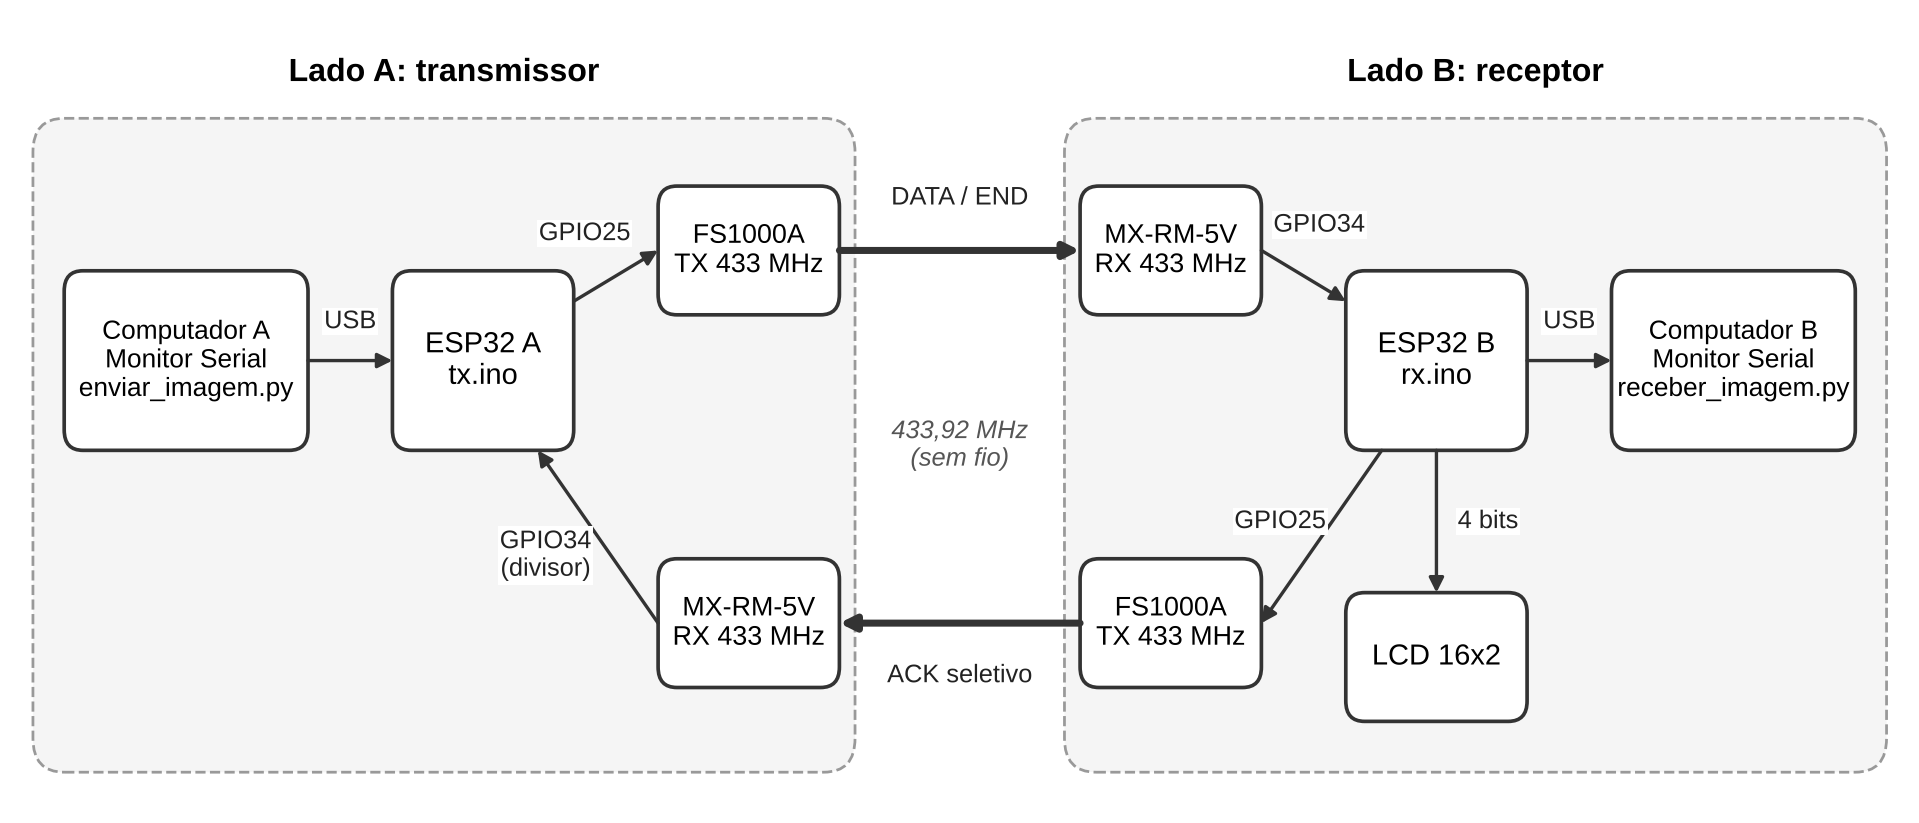
\includegraphics[width=15.5cm]{fig/diagrama_blocos.png}
  \fonte{Elaborado pelos autores (2026).}
\end{figure}

\section{Materiais}

A Tabela 3 relaciona os componentes utilizados nas duas placas.

\begin{table}[H]
  \centering
  \caption{Materiais utilizados}
  \small\renewcommand{\arraystretch}{1.3}
  \begin{tabular}{|>{\raggedright\arraybackslash}m{6.96cm}|>{\centering\arraybackslash}m{2.38cm}|>{\centering\arraybackslash}m{5.31cm}|}
  \hline
  \rowcolor{gray!22}\textbf{Item} & \textbf{Quantidade} & \textbf{Observação} \\ \hline
  ESP32 DevKit V1 (WROOM-32, 30 pinos, USB-C) & 2 & Uma por lado do enlace \\ \hline
  Transmissor de 433 MHz FS1000A & 2 & Um por placa \\ \hline
  Receptor de 433 MHz MX-RM-5V & 2 & Um por placa \\ \hline
  LCD 16x2 paralelo (controlador HD44780) & 1 & Somente na placa B \\ \hline
  Potenciômetro de 10 kΩ & 1 & Ajuste de contraste do LCD \\ \hline
  Resistor de 10 kΩ & 6 & Três por placa, no divisor de tensão \\ \hline
  Fio rígido de 17,3 cm & 4 & Antena de cada módulo \\ \hline
  \textit{Protoboard} de 830 furos & 2 & Uma por placa \\ \hline
  \textit{Jumpers} macho-macho & cerca de 30 & Ligações \\ \hline
  \textit{Jumpers} macho-fêmea & 3 & Ligação do potenciômetro, cujos terminais não encaixam diretamente na \textit{protoboard} \\ \hline
  Computador com Arduino IDE 2 e Python 3 & 2 & Um por placa, conforme o enunciado \\ \hline
  \end{tabular}
  \fonte{Elaborado pelos autores (2026).}
\end{table}

\section{Montagem do hardware}

As duas placas possuem a mesma montagem de rádio, descrita na Tabela 4. Como a ESP32 de 30 pinos ocupa toda a largura útil de um lado da \textit{protoboard}, todos os pinos utilizados foram escolhidos do lado que permanece acessível.

\begin{table}[H]
  \centering
  \caption{Ligações dos módulos de rádio (iguais nas duas placas)}
  \small\renewcommand{\arraystretch}{1.3}
  \begin{tabular}{|>{\raggedright\arraybackslash}m{3.30cm}|>{\centering\arraybackslash}m{6.04cm}|>{\centering\arraybackslash}m{5.31cm}|}
  \hline
  \rowcolor{gray!22}\textbf{Pino da ESP32} & \textbf{Ligação} & \textbf{Função} \\ \hline
  VIN (5 V do USB) & VCC do FS1000A e do MX-RM-5V & Alimentação dos rádios \\ \hline
  GND & GND dos dois módulos & Referência \\ \hline
  D25 (GPIO25) & DATA do FS1000A & Saída da UART2 para o rádio \\ \hline
  D34 (GPIO34) & DATA do MX-RM-5V, por divisor de tensão & Entrada da UART2 \\ \hline
  \end{tabular}
  \fonte{Elaborado pelos autores (2026).}
\end{table}

O receptor MX-RM-5V exige alimentação de 5 V e sua saída acompanha esse nível, enquanto as entradas da ESP32 admitem no máximo 3,3 V. Utilizou-se um divisor resistivo com R1 = 10 kΩ e R2 = 20 kΩ, este formado por dois resistores de 10 kΩ em série, que fornece a tensão da Equação 4.

\begin{equation}
  V_{\text{GPIO}} = 5\ \text{V} \cdot \frac{R_{2}}{R_{1} + R_{2}} = 5 \cdot \frac{20}{30} = 3{,}33\ \text{V}
\end{equation}

As antenas são fios retos de um quarto do comprimento de onda, soldados no terminal ANT de cada módulo, com o comprimento dado pela Equação 5.

\begin{equation}
  \frac{\lambda}{4} = \frac{c}{4f} = \frac{3 \times 10^{8}}{4 \times 433{,}92 \times 10^{6}} \approx 17{,}3\ \text{cm}
\end{equation}

A placa B recebeu ainda o LCD 16x2, operado no modo de 4 bits pela biblioteca LiquidCrystal, com as ligações da Tabela 5. A Figura 2 reúne essas ligações no esquema elétrico completo de uma placa; no esquema, R2 aparece como os dois resistores de 10 kΩ em série (R2a e R2b). As Figuras 3 a 6 mostram a montagem final.

\begin{table}[H]
  \centering
  \caption{Ligações do LCD na placa B}
  \small\renewcommand{\arraystretch}{1.3}
  \begin{tabular}{|>{\raggedright\arraybackslash}m{5.66cm}|>{\centering\arraybackslash}m{9.44cm}|}
  \hline
  \rowcolor{gray!22}\textbf{Pino do LCD} & \textbf{Ligação} \\ \hline
  1 (VSS), 5 (RW), 16 (K) & GND \\ \hline
  2 (VDD), 15 (A) & 5 V \\ \hline
  3 (V0) & Terminal central do potenciômetro \\ \hline
  4 (RS) e 6 (E) & D13 e D14 \\ \hline
  11 a 14 (D4 a D7) & D27, D26, D33 e D32 \\ \hline
  7 a 10 (D0 a D3) & Sem ligação \\ \hline
  \end{tabular}
  \fonte{Elaborado pelos autores (2026).}
\end{table}

\begin{landscape}
\begin{figure}[p]
  \centering
  \caption{Esquema elétrico das placas (circuito de rádio idêntico em A e B; LCD e potenciômetro somente em B)}
  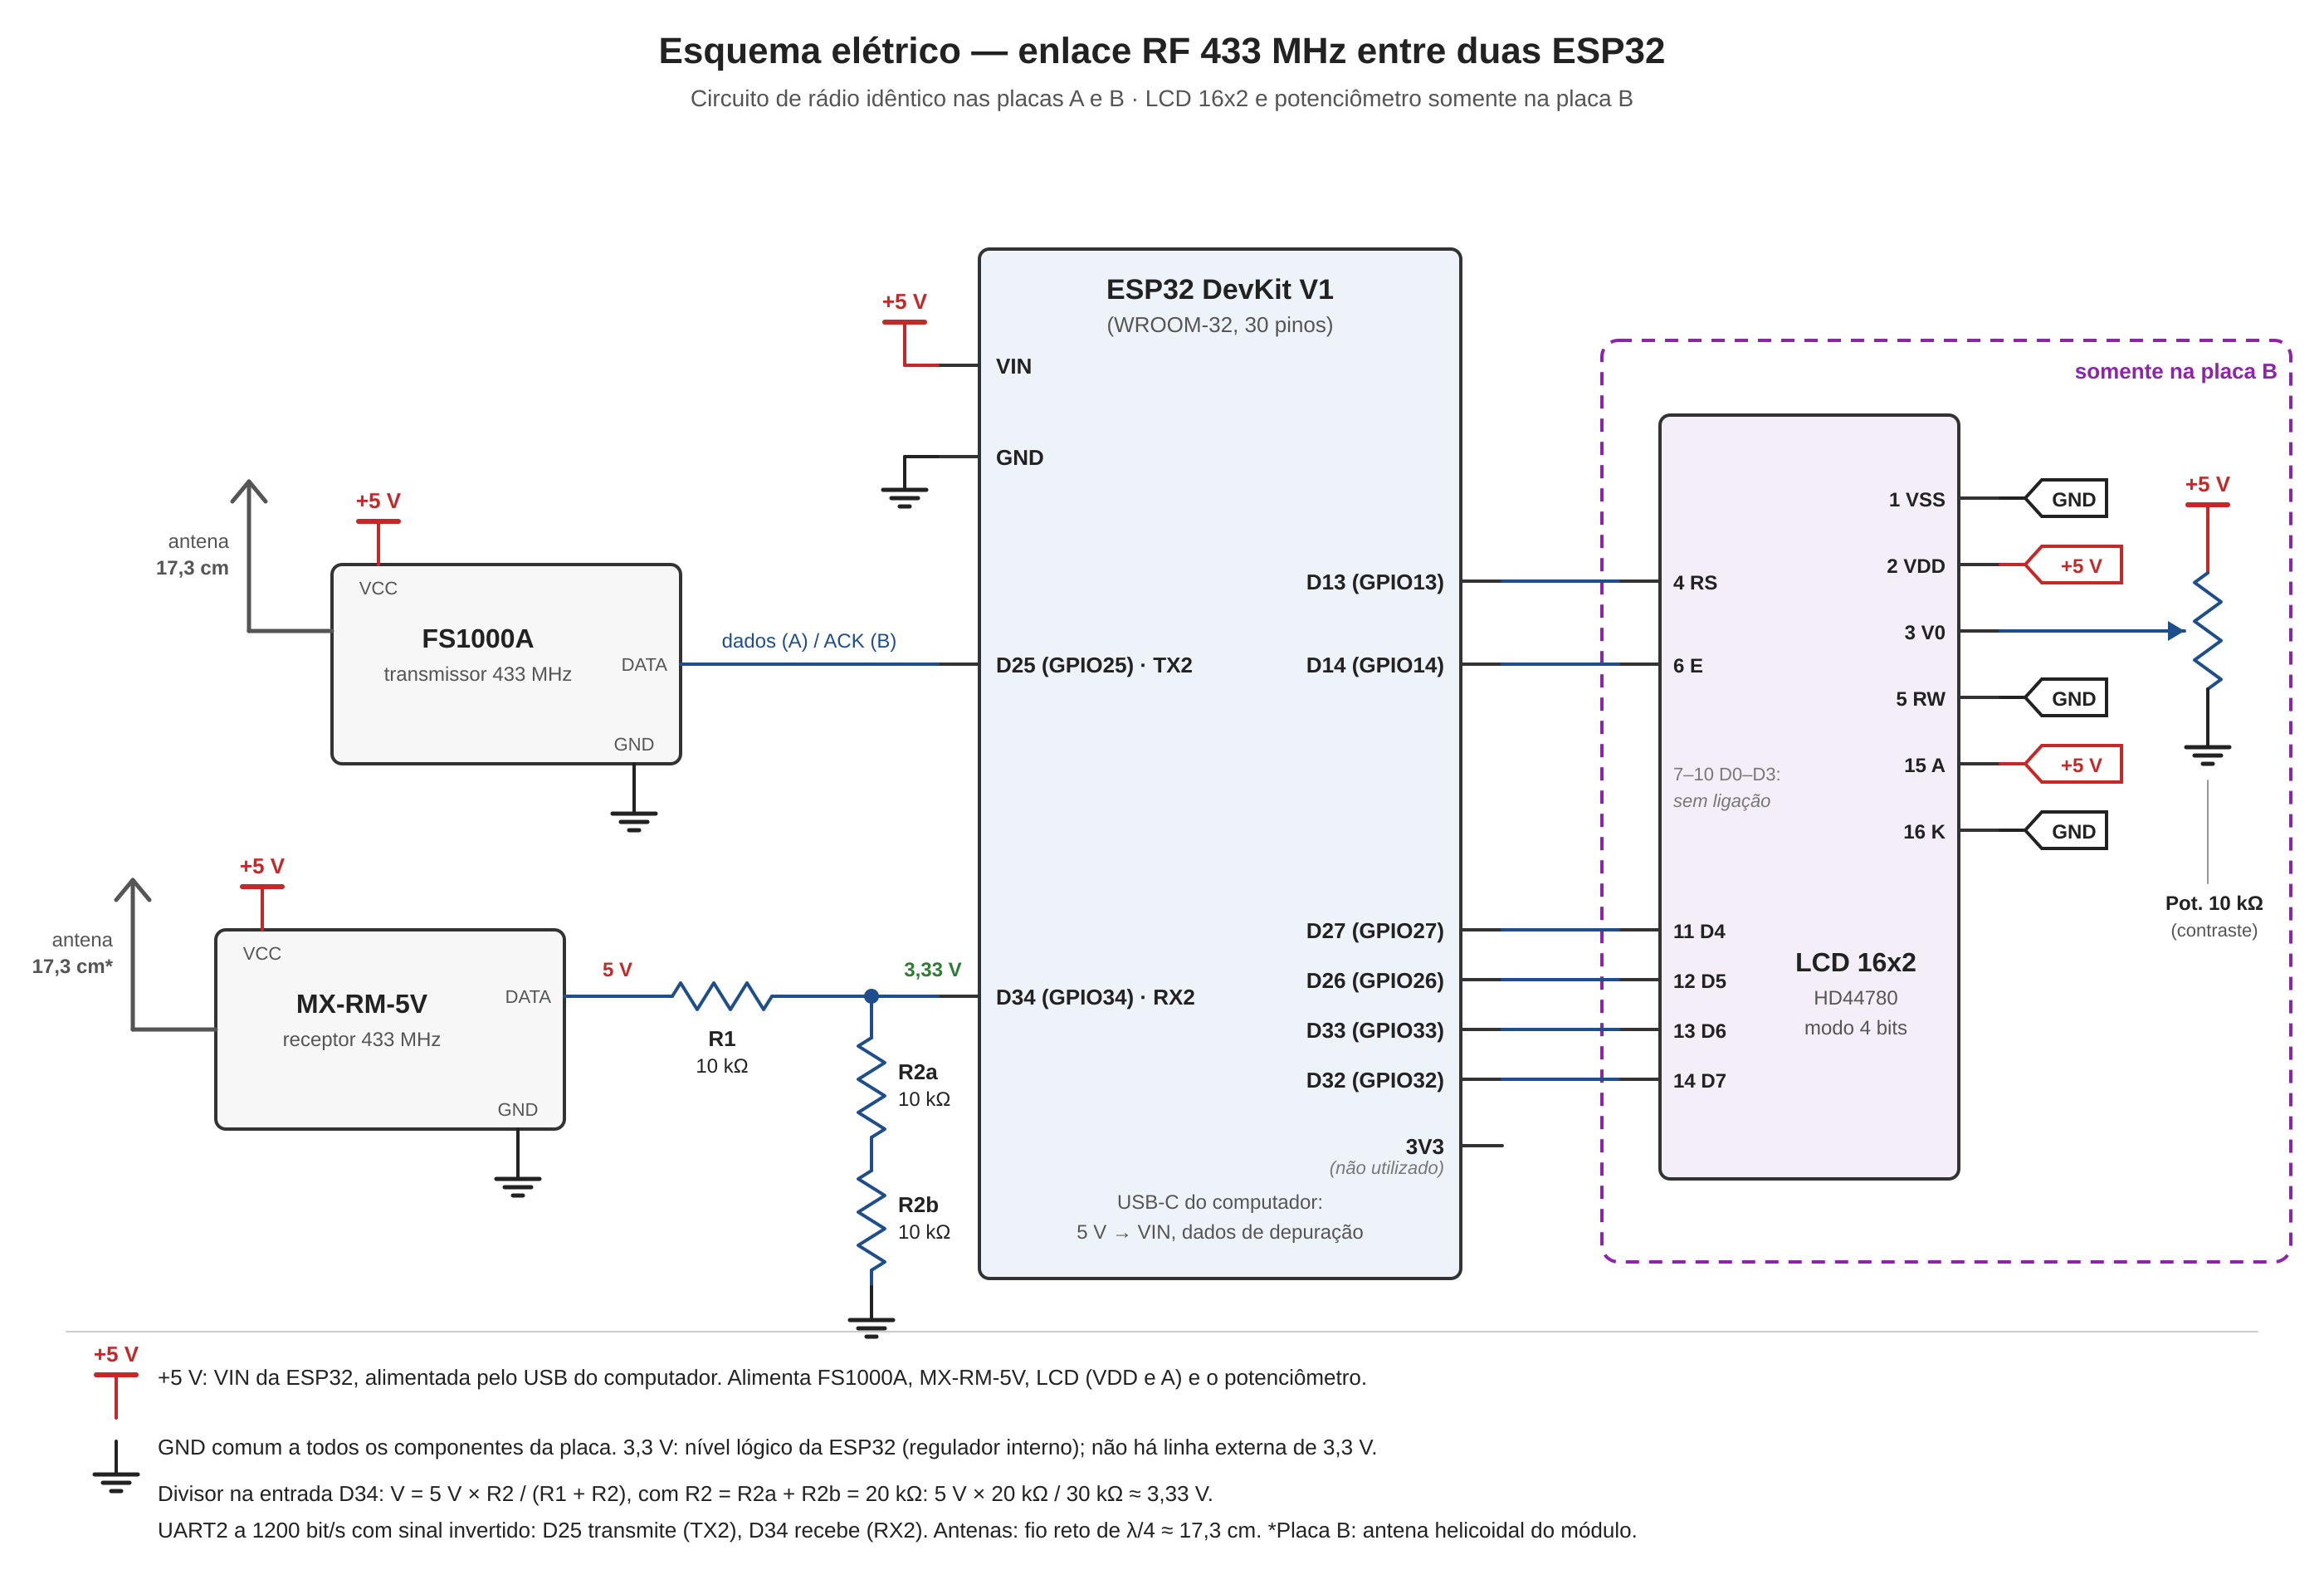
\includegraphics[width=21.0cm]{fig/esquema_eletrico.png}
  \fonte{Elaborado pelos autores (2026).}
\end{figure}
\end{landscape}

\begin{figure}[H]
  \centering
  \caption{Bancada com a placa B (à esquerda) e a placa A (à direita)}
  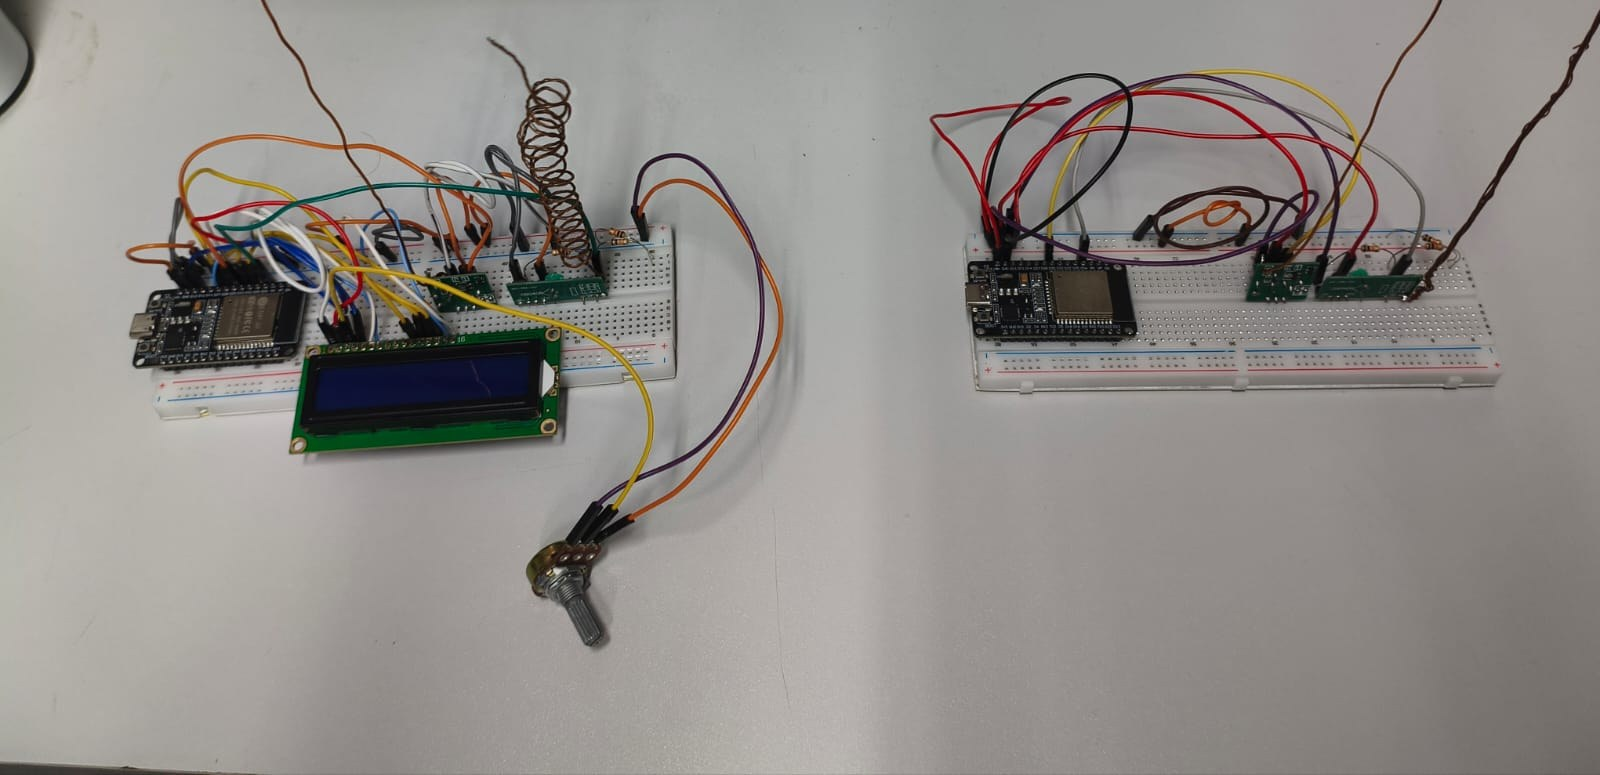
\includegraphics[width=15.5cm]{fig/foto_bancada.jpg}
  \fonte{Elaborado pelos autores (2026).}
\end{figure}

\begin{figure}[H]
  \centering
  \caption{Placa A (transmissor) com os módulos de rádio e o divisor de tensão}
  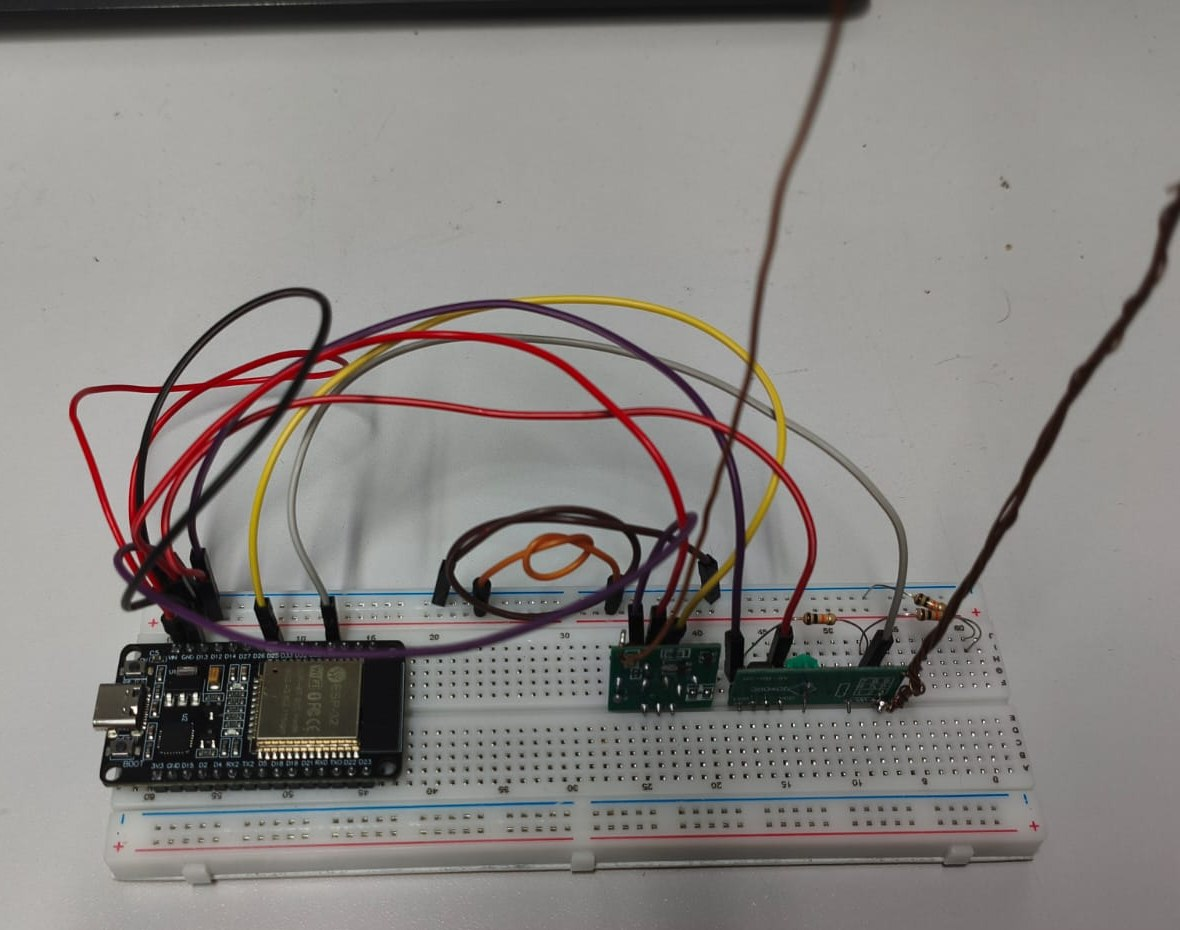
\includegraphics[width=13.0cm]{fig/foto_placa_a.jpg}
  \fonte{Elaborado pelos autores (2026).}
\end{figure}

\begin{figure}[H]
  \centering
  \caption{Placa B (receptor) com o LCD 16x2 e o potenciômetro de contraste}
  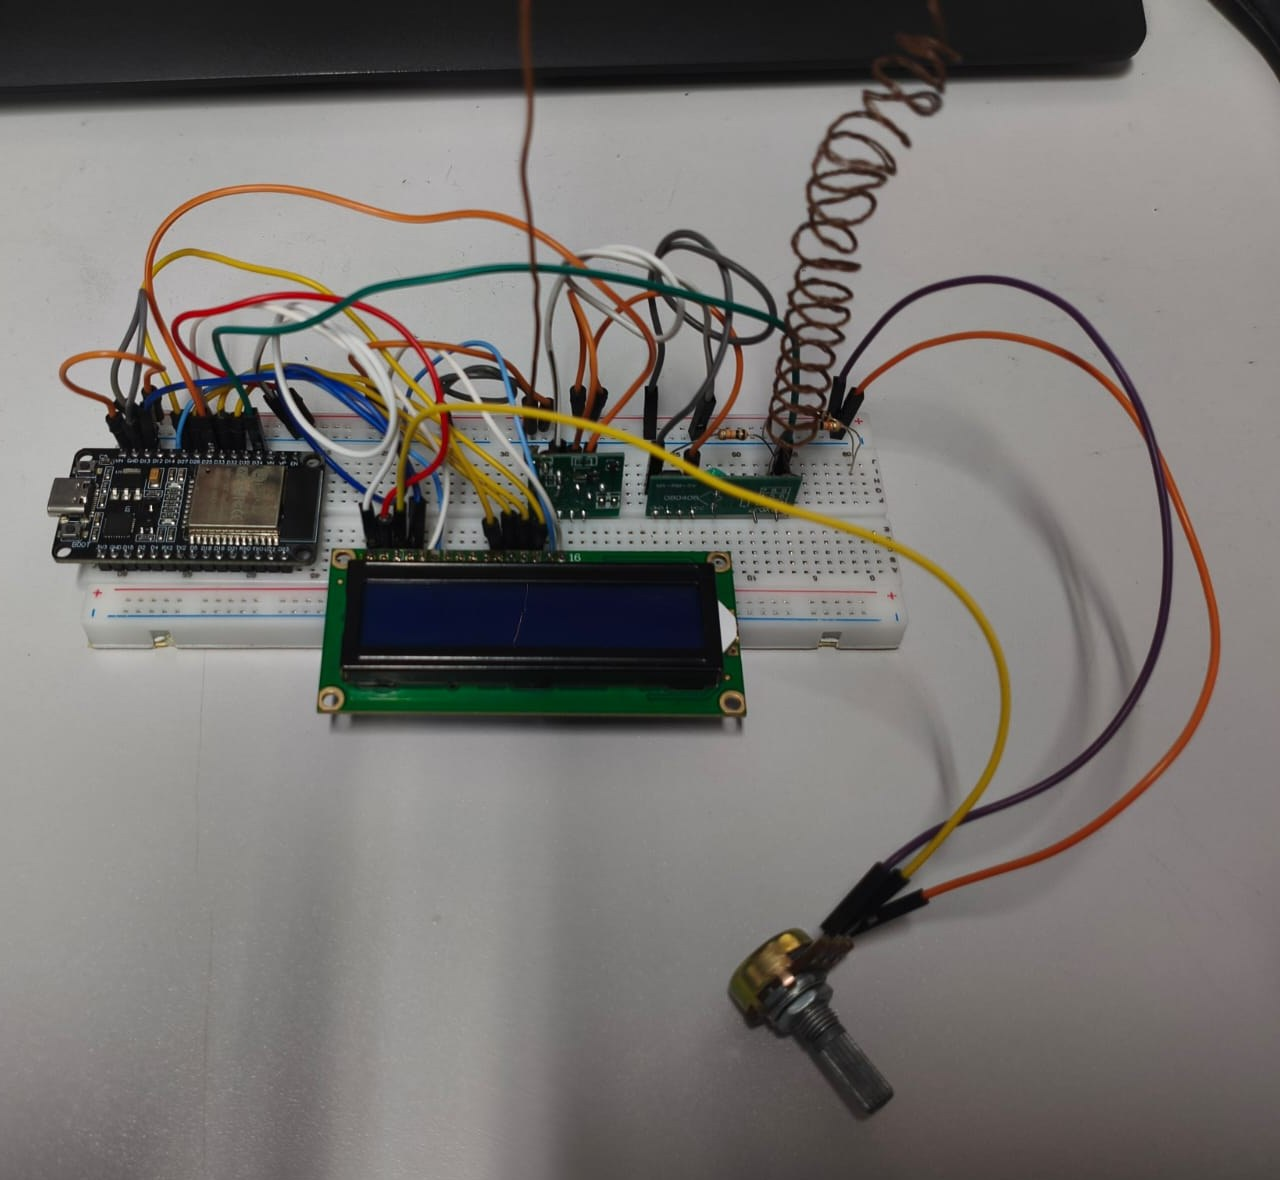
\includegraphics[width=13.0cm]{fig/foto_placa_b.jpg}
  \fonte{Elaborado pelos autores (2026).}
\end{figure}

\begin{figure}[H]
  \centering
  \caption{Detalhe dos módulos FS1000A e MX-RM-5V na placa A}
  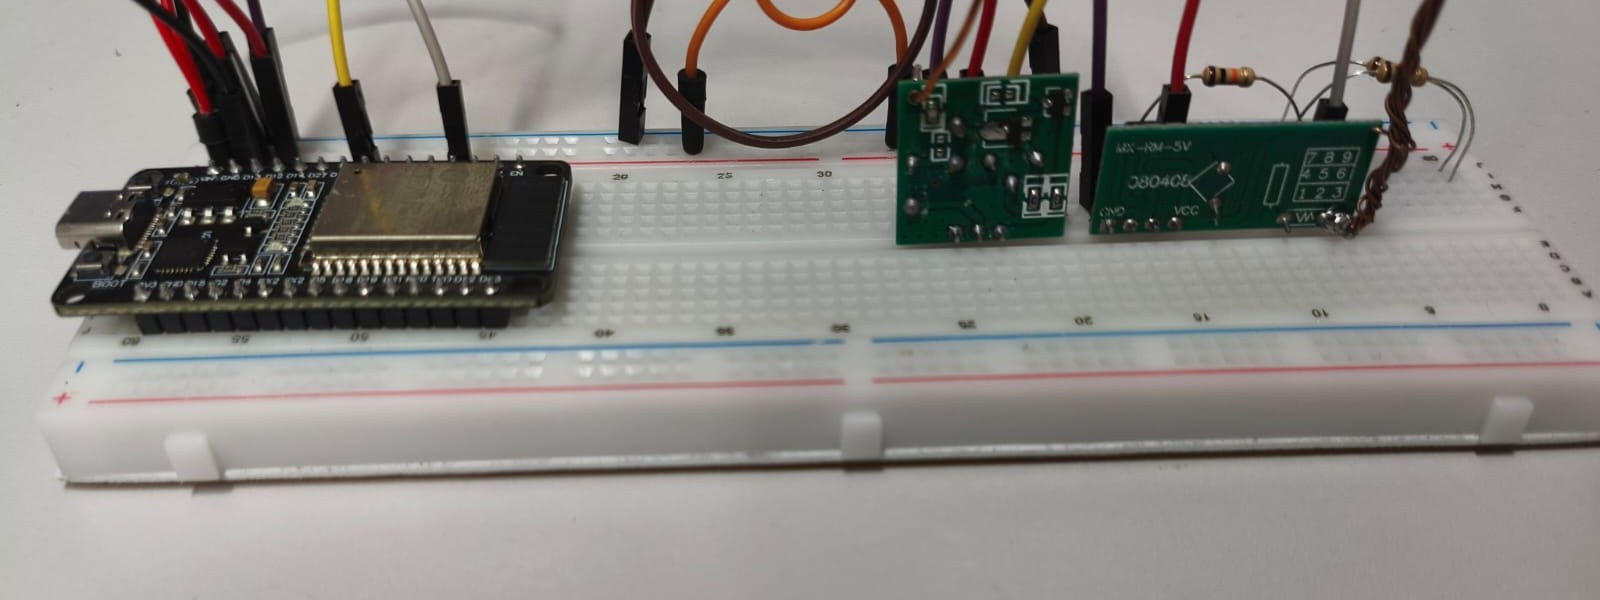
\includegraphics[width=14.0cm]{fig/foto_modulos.jpg}
  \fonte{Elaborado pelos autores (2026).}
\end{figure}

\section{Estrutura do quadro}

O quadro segue a estrutura definida no enunciado e possui no máximo 21 bytes. A Tabela 6 descreve os campos; quadros com TYPE diferente dos três valores previstos ou com LEN superior a 16 são descartados pelo receptor.

\begin{table}[H]
  \centering
  \caption{Campos do quadro}
  \small\renewcommand{\arraystretch}{1.3}
  \begin{tabular}{|>{\raggedright\arraybackslash}m{2.20cm}|>{\centering\arraybackslash}m{2.75cm}|>{\centering\arraybackslash}m{9.71cm}|}
  \hline
  \rowcolor{gray!22}\textbf{Campo} & \textbf{Tamanho} & \textbf{Conteúdo} \\ \hline
  FLAG & 1 byte & 0x7E, início do quadro \\ \hline
  TYPE & 1 byte & 0x01 = DATA; 0x02 = ACK; 0x03 = END \\ \hline
  SEQ & 1 byte & Número de sequência, de 0 a 255 \\ \hline
  LEN & 1 byte & Quantidade de bytes em DATA, de 0 a 16 \\ \hline
  DATA & 0 a 16 bytes & Carga útil \\ \hline
  FCS & 1 byte & CRC-8 calculado sobre TYPE, SEQ, LEN e DATA \\ \hline
  \end{tabular}
  \fonte{Elaborado pelos autores com base em IFMT (2026).}
\end{table}

O quadro DATA transporta até 16 bytes da mensagem, cujo primeiro byte identifica o conteúdo: T para texto e I para imagem. O quadro ACK transporta em SEQ o número do próximo quadro esperado em ordem e, no primeiro byte de DATA, um mapa de bits dos quadros já armazenados à frente. O quadro END, com LEN igual a zero, encerra a mensagem e só é enviado depois que todos os quadros DATA foram confirmados.

\section{Cálculo do FCS}

O FCS é um CRC-8 com polinômio 0x07, valor inicial 0x00, sem reflexão de bits e sem XOR final, parâmetros que correspondem ao CRC-8/SMBUS catalogado por Cook (2026), cujo valor de verificação para a sequência ASCII 123456789 é 0xF4; a implementação reproduz esse valor. O cálculo abrange TYPE, SEQ, LEN e DATA, excluindo FLAG e o próprio FCS, conforme o enunciado. A implementação processa um byte por vez: o byte entra no registrador por XOR e, em seguida, executam-se oito deslocamentos à esquerda; sempre que o bit descartado é 1, aplica-se XOR com 0x07, o que corresponde à divisão polinomial da Equação 2 realizada bit a bit.

\begin{Verbatim}[fontsize=\scriptsize,frame=single,framesep=2mm,rulecolor=\color{gray!60},breaklines,breakanywhere]
uint8_t crc8(const uint8_t *p, size_t n) {
  uint8_t crc = 0x00;                     // valor inicial
  for (size_t i = 0; i < n; ++i) {
    crc ^= p[i];                          // entra o próximo byte
    for (uint8_t b = 0; b < 8; ++b)       // oito passos da divisão
      crc = (crc & 0x80) ? (crc << 1) ^ 0x07 : (crc << 1);
  }
  return crc;                             // resto = FCS
}
\end{Verbatim}

A Tabela 7 apresenta o cálculo passo a passo para um quadro DATA com SEQ igual a 0 e o texto Oi, cujos bytes protegidos são 01 00 02 4F 69. O transmissor envia FCS = 0x34; o receptor recalcula o valor sobre os bytes recebidos e aceita o quadro somente se obtiver o mesmo resultado.

\begin{table}[H]
  \centering
  \caption{Cálculo do CRC-8 para o quadro DATA com o texto Oi}
  \small\renewcommand{\arraystretch}{1.3}
  \begin{tabular}{|>{\raggedright\arraybackslash}m{4.58cm}|>{\centering\arraybackslash}m{5.04cm}|>{\centering\arraybackslash}m{5.04cm}|}
  \hline
  \rowcolor{gray!22}\textbf{Byte processado} & \textbf{Registrador após o XOR} & \textbf{Registrador após os 8 passos} \\ \hline
  01 (TYPE) & 01 & 07 \\ \hline
  00 (SEQ) & 07 & 15 \\ \hline
  02 (LEN) & 17 & 65 \\ \hline
  4F (O) & 2A & D6 \\ \hline
  69 (i) & BF & 34 \\ \hline
  \end{tabular}
  \fonte{Elaborado pelos autores (2026).}
\end{table}

\section{Camada física}

A camada física foi implementada no próprio \textit{firmware}. Cada quadro é transmitido como um preâmbulo de bytes 0xF0, seguido do delimitador 0x7E e dos campos do quadro codificados em Manchester, de modo que cada byte do quadro ocupa dois bytes na linha. As decisões adotadas foram as seguintes:

\begin{enumerate}[label=\alph*),leftmargin=1.9cm,itemsep=2pt]
  \item UART2 a 1200 bit/s ligada ao pino DATA dos rádios; a 2400 bit/s, o receptor deformava os pulsos e o alcance limitava-se a cerca de 70 cm;
  \item UART com sinal invertido, de modo que o estado de repouso desligue a portadora; sem a inversão, o nível 1 de repouso manteria o transmissor permanentemente ativo e bloquearia as confirmações;
  \item preâmbulo de bytes 0xF0, que na linha produzem metade dos bits em 0 e metade em 1, permitindo o ajuste do ganho do receptor e o alinhamento da UART receptora;
  \item codificação Manchester por \textit{nibble}, com descarte imediato de qualquer byte fora do código;
  \item descarte do eco: como o receptor de cada placa capta o próprio transmissor, os bytes recebidos durante a transmissão são ignorados.
\end{enumerate}

A Tabela 8 resume o tamanho de cada tipo de quadro na linha e o tempo de transmissão correspondente.

\begin{table}[H]
  \centering
  \caption{Tamanho dos quadros na linha a 1200 bit/s}
  \small\renewcommand{\arraystretch}{1.3}
  \begin{tabular}{|>{\raggedright\arraybackslash}m{3.91cm}|>{\centering\arraybackslash}m{4.08cm}|>{\centering\arraybackslash}m{2.84cm}|>{\centering\arraybackslash}m{3.37cm}|}
  \hline
  \rowcolor{gray!22}\textbf{Quadro} & \textbf{Composição na linha} & \textbf{Bytes na linha} & \textbf{Tempo no ar} \\ \hline
  DATA com 16 bytes & 8 + 1 + 2 × 20 & 49 & 408 ms \\ \hline
  END & 8 + 1 + 2 × 4 & 17 & 142 ms \\ \hline
  ACK & 48 + 1 + 2 × 5 & 59 & 492 ms \\ \hline
  \end{tabular}
  \fonte{Elaborado pelos autores (2026).}
\end{table}

\section{Selective Repeat}

O transmissor divide a mensagem em quadros DATA numerados a partir de zero e envia uma rajada de até W quadros novos, com W igual a 4 por padrão e ajustável de 1 a 8. Ao término da rajada, interrompe a transmissão e aguarda a confirmação. Ao receber um ACK, marca como confirmados todos os quadros anteriores ao valor de SEQ e os quadros indicados no mapa de bits. Um quadro enviado antes desse ACK e que não consta nele é considerado perdido e retransmitido imediatamente, de modo que o ACK seletivo desempenha também a função de confirmação negativa. Na ausência de ACK, cada quadro possui um temporizador próprio de 1117 ms e, ao expirar, apenas aquele quadro é retransmitido.

O receptor mantém uma janela de 8 posições a partir do próximo número de sequência esperado. Quadros dentro da janela e com CRC correto são armazenados; quando o quadro esperado chega, ele e os seguintes já armazenados são entregues em ordem. Quadros já entregues são descartados e provocam a repetição do ACK. Após 425 ms de silêncio no canal, o receptor envia um único ACK para a rajada, com SEQ igual ao próximo quadro esperado e DATA[0] contendo o mapa de bits, no qual o bit i indica que o quadro SEQ + i já foi armazenado.

A Tabela 9 reúne os tempos do protocolo, todos calculados no \textit{firmware} a partir da taxa de transmissão. O silêncio que antecede o ACK precisa ser maior que o intervalo entre dois quadros de uma mesma rajada; caso contrário, o receptor responderia no meio dela. O acréscimo de 300 ms e o preâmbulo de 48 bytes no ACK decorrem de uma limitação observada em bancada: logo após transmitir, o receptor da placa A, situado a poucos centímetros do próprio transmissor, permanece com ganho reduzido e demora a detectar um sinal fraco vindo da outra placa.

\begin{table}[H]
  \centering
  \caption{Tempos do protocolo a 1200 bit/s}
  \small\renewcommand{\arraystretch}{1.3}
  \begin{tabular}{|>{\raggedright\arraybackslash}m{6.04cm}|>{\centering\arraybackslash}m{5.13cm}|>{\centering\arraybackslash}m{3.48cm}|}
  \hline
  \rowcolor{gray!22}\textbf{Parâmetro} & \textbf{Expressão} & \textbf{Valor} \\ \hline
  Tempo de um byte & 10 / 1200 s & 8,33 ms \\ \hline
  Silêncio antes do ACK & (8 + 4) × 8,33 + 25 + 300 & 425 ms \\ \hline
  Duração do ACK & 59 × 8,33 + 1 & 492 ms \\ \hline
  Temporizador de cada quadro & 425 + 492 + 200 & 1117 ms \\ \hline
  Intervalo entre mensagens & temporizador + 300 & 1417 ms \\ \hline
  Desistência do transmissor & sem confirmação nova & 20 s \\ \hline
  Descarte de mensagem incompleta no receptor & sem quadro válido & 26 s \\ \hline
  \end{tabular}
  \fonte{Elaborado pelos autores (2026).}
\end{table}

Casos de borda também foram tratados. Se o ACK do quadro END se perder, o receptor reconhece o END repetido e confirma novamente sem entregar a mensagem duas vezes. Cada mensagem recomeça em SEQ 0, e o intervalo de 1417 ms entre mensagens impede que um ACK atrasado seja atribuído à mensagem seguinte. Como a desistência do transmissor ocorre antes do descarte no receptor, as duas placas retornam juntas ao estado inicial após uma queda do enlace.

\section{Firmware e ferramentas de apoio}

O \textit{firmware} foi desenvolvido na Arduino IDE 2 com o pacote ESP32 da Espressif e dividido em três arquivos. O arquivo protocolo\_rf.h, presente em cópias idênticas nas duas placas, contém os tempos, a estrutura do quadro, o CRC-8, a codificação Manchester e o receptor de linha. O arquivo tx.ino implementa a segmentação da mensagem, o \textit{Selective Repeat} do transmissor e a recepção de imagens pelo USB; o arquivo rx.ino implementa a janela do receptor, a entrega em ordem, os ACKs, o LCD e a saída da imagem para o computador. A Tabela 10 lista os comandos disponíveis no Monitor Serial.

\begin{table}[H]
  \centering
  \caption{Comandos disponíveis no Monitor Serial}
  \small\renewcommand{\arraystretch}{1.3}
  \begin{tabular}{|>{\raggedright\arraybackslash}m{4.21cm}|>{\centering\arraybackslash}m{1.83cm}|>{\centering\arraybackslash}m{8.61cm}|}
  \hline
  \rowcolor{gray!22}\textbf{Comando} & \textbf{Placa} & \textbf{Função} \\ \hline
  texto + Enter & A & Envia o texto \\ \hline
  /janela N & A & Define a janela de 1 a 8 (1 equivale ao Stop-and-Wait) \\ \hline
  /erro P & A & Inverte 1 bit em P\% dos quadros após o cálculo do CRC \\ \hline
  /perda P & A & Deixa de transmitir P\% dos quadros \\ \hline
  /teste N & A & Envia uma mensagem de teste com N caracteres \\ \hline
  /imagem N & A & Recebe N bytes pelo USB e os transmite como imagem \\ \hline
  /status, /resumo, /bench & A e B & Estado, totais da sessão e tempo médio do CRC \\ \hline
  /reinicia & B & Retorna o receptor ao estado inicial \\ \hline
  \end{tabular}
  \fonte{Elaborado pelos autores (2026).}
\end{table}

O comando /erro atua sobre o quadro depois do cálculo do FCS e antes da codificação Manchester. Assim, o erro chega ao receptor com codificação de linha válida e somente o CRC pode detectá-lo, o que permite demonstrar a detecção de forma isolada. Cada evento do enlace gera uma linha no Monitor Serial, com o instante em milissegundos, os bytes do quadro em hexadecimal, o FCS recebido e o calculado e o tempo de cálculo do CRC em microssegundos.

No computador, três \textit{scripts} em Python completam o sistema: enviar\_imagem.py transfere a imagem para a placa A; receber\_imagem.py reconstrói o arquivo a partir da saída da placa B e calcula o resumo SHA-256; e coletar\_testes.py executa a bateria de ensaios, grava os \textit{logs} das duas placas e gera planilhas CSV com os resultados.

\section{Procedimento de ensaio}

Os ensaios foram realizados em 21/11/2026, entre 12h58 e 13h47, em ambiente interno, com o \textit{firmware} na versão 4.1. As duas placas foram ligadas ao mesmo notebook, operando com bateria, para que o script de coleta registrasse os \textit{logs} do transmissor e do receptor com a mesma referência de tempo e associasse cada ensaio aos dois lados do enlace. A ligação USB serviu apenas para alimentação e registro; não houve nenhum condutor de dados entre as placas, e toda a comunicação ocorreu pelo rádio. A configuração final do enunciado, com uma placa em cada computador, foi verificada em 23/11/2026, conforme a Seção 4.7. Durante a campanha, as antenas permaneceram retas, verticais e paralelas, e a distância foi medida entre as antenas. A mensagem padrão foi gerada pelo comando /teste 200, que produz 201 bytes, isto é, 13 quadros DATA e um END. O ensaio de ruído utilizou 500 caracteres e o de imagem utilizou um arquivo PNG de 32 × 32 pixels com 490 bytes. Cada cenário da Tabela 11 foi repetido três vezes, totalizando 36 ensaios.

\begin{table}[H]
  \centering
  \caption{Cenários de ensaio}
  \small\renewcommand{\arraystretch}{1.3}
  \begin{tabular}{|>{\raggedright\arraybackslash}m{3.19cm}|>{\centering\arraybackslash}m{5.86cm}|>{\centering\arraybackslash}m{2.48cm}|>{\centering\arraybackslash}m{2.66cm}|}
  \hline
  \rowcolor{gray!22}\textbf{Grupo} & \textbf{Cenário} & \textbf{Distância} & \textbf{Janela} \\ \hline
  Distância & 0,5 m, 1 m, 1,5 m e 2 m & variável & 4 \\ \hline
  Janela & 1 (Stop-and-Wait), 4 e 8 & 1 m & variável \\ \hline
  Erro simulado & /erro 30 & 1 m & 4 \\ \hline
  Perda simulada & /perda 30 & 1 m & 4 \\ \hline
  Ruído real & celular encostado no receptor & 1 m & 4 \\ \hline
  Imagem & sem erro e com /erro 30 & 1 m & 4 \\ \hline
  \end{tabular}
  \fonte{Elaborado pelos autores (2026).}
\end{table}

Considerou-se entregue o ensaio em que o transmissor registrou a entrega e o conteúdo apresentado pelo receptor coincidiu integralmente com o enviado; para imagens, exigiu-se a igualdade do resumo SHA-256. Considerou-se falha o ensaio em que o transmissor abandonou a mensagem após 20 s sem confirmação.

Em 23/11/2026, os grupos de distância e de janela foram repetidos com uma placa em cada computador, três vezes por cenário, totalizando 21 ensaios. O script de coleta foi executado no modo tx no computador A e no modo rx no computador B; ao final, o modo juntar associou os registros dos dois lados pelo tamanho da mensagem e pelo horário, com correção automática da diferença entre os relógios dos computadores, estimada em 0,66 s. Na mesma data, foram transmitidas duas imagens a 1,8 m e registrados o resumo da sessão e o tempo do CRC, descritos na Seção 4.7.


\chapter{RESULTADOS E DISCUSSÃO}
Dos 36 ensaios, 33 resultaram em entrega (91,7\%) e nenhum resultou em entrega com conteúdo diferente do enviado. As três falhas corresponderam a mensagens abandonadas pelo transmissor após 20 s sem confirmação. Nas tabelas a seguir, tempo e número de retransmissões são médias dos ensaios entregues.

\section{Distância}

\begin{table}[H]
  \centering
  \caption{Resultados por distância (janela 4, mensagem de 201 bytes)}
  \small\renewcommand{\arraystretch}{1.3}
  \begin{tabular}{|>{\raggedright\arraybackslash}m{2.23cm}|>{\centering\arraybackslash}m{2.23cm}|>{\centering\arraybackslash}m{2.58cm}|>{\centering\arraybackslash}m{2.92cm}|>{\centering\arraybackslash}m{3.78cm}|}
  \hline
  \rowcolor{gray!22}\textbf{Distância} & \textbf{Entregues} & \textbf{Tempo médio} & \textbf{Retransmissões} & \textbf{ACKs enviados / recebidos} \\ \hline
  0,5 m & 3 de 3 & 10,3 s & 0 & 15 / 15 \\ \hline
  1,0 m & 2 de 3 & 13,9 s & 2,5 & 24 / 12 \\ \hline
  1,5 m & 2 de 3 & 29,9 s & 18 & 37 / 19 \\ \hline
  2,0 m & 3 de 3 & 19,8 s & 8 & 22 / 20 \\ \hline
  \end{tabular}
  \fonte{Elaborado pelos autores a partir dos \textit{logs} de 21/11/2026.}
\end{table}

O enlace funcionou até 2 m, o dobro da distância mínima exigida. A 0,5 m, as três entregas levaram 10,26 s, sem retransmissões. A última coluna da Tabela 12 identifica a origem das perdas: a 1 m e a 1,5 m, cerca de metade dos ACKs enviados pelo receptor não chegou ao transmissor. Os dados alcançavam a placa B, mas a confirmação se perdia no sentido inverso, o que levava o transmissor a retransmitir por estouro do temporizador. As três falhas da bateria tiveram essa mesma causa.

O desempenho não decresceu de forma monotônica com a distância, já que o ensaio a 2 m superou os de 1 m e 1,5 m. Em ambiente interno, o sinal de 433 MHz chega ao receptor por múltiplos percursos, refletido por paredes e objetos, e a posição exata das placas influencia o resultado tanto quanto a distância. Além disso, os cenários foram executados em instantes diferentes, sob condições de ruído que variam ao longo do tempo.

\section{Comparação entre tamanhos de janela}

Para estimar o tempo em canal sem perdas, adotou-se um modelo simples: cada quadro DATA completo ocupa cerca de 437 ms, somados o tempo no ar e o descarte do eco, e cada rajada termina com cerca de 900 ms de espera pelo ACK, conforme a Equação 6, em que k é o número de quadros da rajada.

\begin{equation}
  T \approx \sum_{\text{rajadas}} \left( k \cdot 437\ \text{ms} + 900\ \text{ms} \right) + T_{\text{END}}
\end{equation}

Para janela 4, o modelo prevê 10,2 s, valor próximo dos 10,26 s medidos a 0,5 m, o que valida o modelo. A Tabela 13 e a Figura 7 comparam as previsões com as medições realizadas a 1 m.

\begin{table}[H]
  \centering
  \caption{Tempo de entrega por tamanho de janela (1 m)}
  \small\renewcommand{\arraystretch}{1.3}
  \begin{tabular}{|>{\raggedright\arraybackslash}m{3.09cm}|>{\centering\arraybackslash}m{2.75cm}|>{\centering\arraybackslash}m{2.58cm}|>{\centering\arraybackslash}m{2.41cm}|>{\centering\arraybackslash}m{2.92cm}|}
  \hline
  \rowcolor{gray!22}\textbf{Janela} & \textbf{Teórico (canal limpo)} & \textbf{Média medida} & \textbf{Melhor caso} & \textbf{Retransmissões} \\ \hline
  1 (Stop-and-Wait) & 18,3 s & 41,5 s & 40,0 s & 15 \\ \hline
  4 & 10,2 s & 26,9 s & 18,8 s & 14 \\ \hline
  8 & 8,4 s & 18,1 s & 12,7 s & 9,7 \\ \hline
  \end{tabular}
  \fonte{Elaborado pelos autores a partir dos \textit{logs} de 21/11/2026.}
\end{table}

\begin{figure}[H]
  \centering
  \caption{Tempo de entrega teórico e medido por tamanho de janela}
  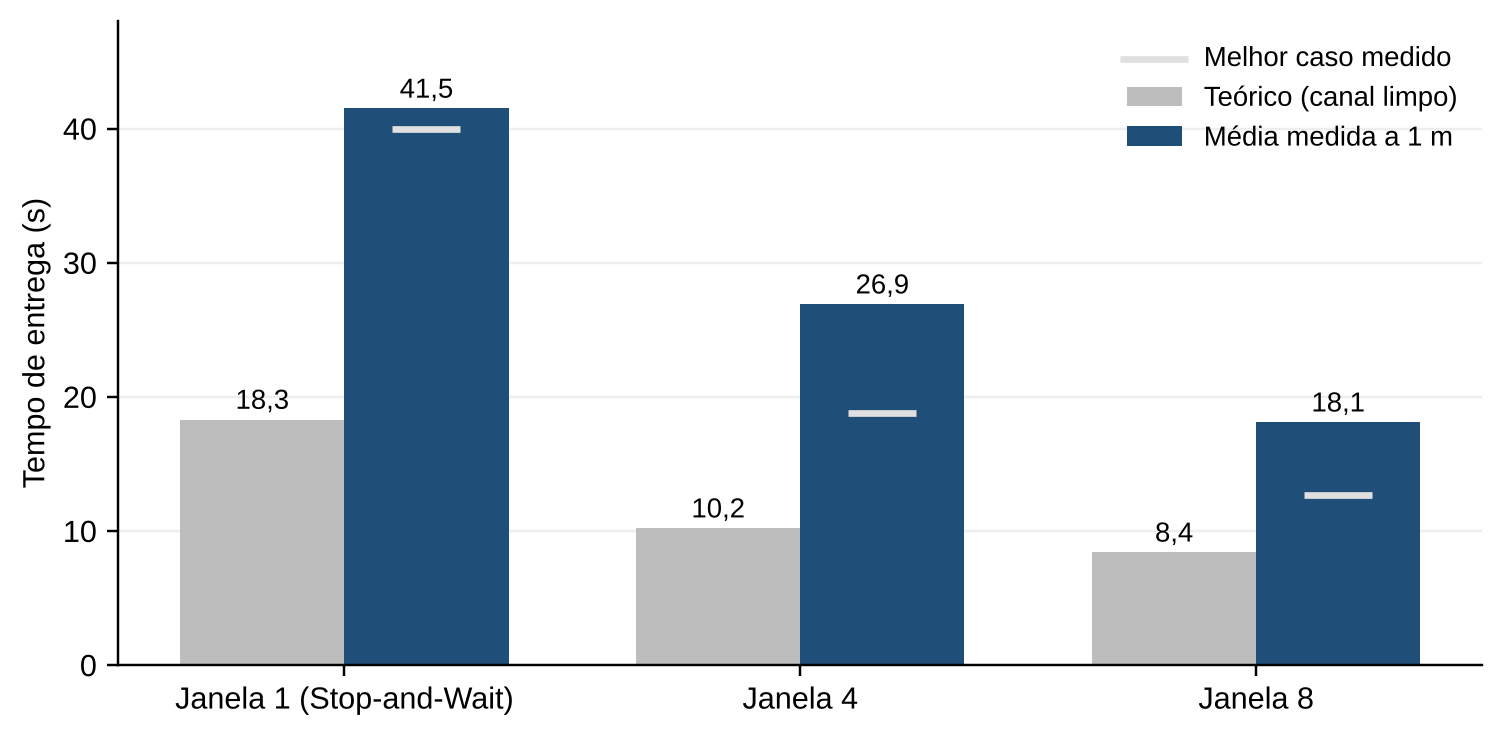
\includegraphics[width=14.0cm]{fig/grafico_janela.png}
  \fonte{Elaborado pelos autores a partir dos \textit{logs} de 21/11/2026.}
\end{figure}

Com janela 8, o \textit{Selective Repeat} entregou as mensagens em média 56\% mais rápido que o \textit{Stop-and-Wait}. No \textit{Stop-and-Wait}, cada quadro paga integralmente a espera de cerca de 900 ms pelo ACK; com janela 8, essa espera é dividida entre oito quadros. Os tempos medidos superaram os teóricos porque, na posição de 1 m, o canal perdia quadros e confirmações. A primeira repetição com janela 4 (43,1 s e 28 retransmissões) coincidiu com um período de pior qualidade do canal; as outras duas levaram 18,8 s.

\section{Erros simulados, perdas simuladas e ruído real}

\begin{table}[H]
  \centering
  \caption{Resultados com erros, perdas e ruído (1 m, janela 4)}
  \small\renewcommand{\arraystretch}{1.3}
  \begin{tabular}{|>{\raggedright\arraybackslash}m{3.44cm}|>{\centering\arraybackslash}m{2.06cm}|>{\centering\arraybackslash}m{2.41cm}|>{\centering\arraybackslash}m{2.92cm}|>{\centering\arraybackslash}m{2.92cm}|}
  \hline
  \rowcolor{gray!22}\textbf{Cenário} & \textbf{Entregues} & \textbf{Tempo médio} & \textbf{Retransmissões} & \textbf{Erros detectados pelo CRC} \\ \hline
  /erro 30 & 3 de 3 & 28,1 s & 14 & 17 \\ \hline
  /perda 30 & 3 de 3 & 41,2 s & 38,3 & 0 \\ \hline
  Ruído real (500 caracteres) & 2 de 3 & 46,9 s & 19 & 0 \\ \hline
  \end{tabular}
  \fonte{Elaborado pelos autores a partir dos \textit{logs} de 21/11/2026.}
\end{table}

Com o erro simulado, todos os quadros corrompidos que chegaram ao receptor foram descartados pelo CRC e retransmitidos, e os três textos chegaram idênticos ao original. Com a perda simulada, 55 quadros deixaram de ser transmitidos e o \textit{Selective Repeat} recuperou todos, retransmitindo apenas os ausentes. Sob ruído real, com um celular encostado ao receptor, as mensagens de 500 caracteres chegaram íntegras, com mais retransmissões. Na segunda repetição desse cenário, além do celular, a antena do receptor foi coberta com a mão; o canal tornou-se inutilizável e o transmissor abandonou a mensagem após 20 s, sem entregar dado incorreto.

\section{Detecção de erros e custo do CRC}

Nenhum quadro com erro foi aceito ao longo da bateria. O receptor descartou quadros com erro em dois níveis, conforme a Tabela 15.

\begin{table}[H]
  \centering
  \caption{Quadros descartados por nível de verificação}
  \small\renewcommand{\arraystretch}{1.3}
  \begin{tabular}{|>{\raggedright\arraybackslash}m{5.86cm}|>{\centering\arraybackslash}m{2.01cm}|>{\centering\arraybackslash}m{6.78cm}|}
  \hline
  \rowcolor{gray!22}\textbf{Nível de descarte} & \textbf{Quadros} & \textbf{Origem do erro} \\ \hline
  Código Manchester inválido (quadro truncado) & 186 & Erros reais do canal de rádio \\ \hline
  CRC-8 diferente do calculado & 57 & Bits invertidos pelo comando /erro \\ \hline
  Quadros aceitos com erro & 0 & – \\ \hline
  \end{tabular}
  \fonte{Elaborado pelos autores a partir dos \textit{logs} de 21/11/2026.}
\end{table}

Os comandos /erro inverteram bits em 83 quadros, dos quais 57 chegaram completos ao receptor e foram rejeitados pelo CRC; os demais foram perdidos ou truncados no próprio canal. Todos foram retransmitidos e entregues corretamente. Um exemplo extraído do \textit{log} do receptor mostra o byte 0x59 recebido como 0xD9, com o bit 7 invertido:

\begin{Verbatim}[fontsize=\scriptsize,frame=single,framesep=2mm,rulecolor=\color{gray!60},breaklines,breakanywhere]
RX quadro DATA seq=6: FCS recebido=0x07 calculado=0x33
   quadro=[01 06 10 52 53 54 55 56 57 58 D9 5A 41 42 43 44 45 46 47 07]
   -> ERRO DETECTADO, descartado
\end{Verbatim}

O tempo de cálculo do CRC-8 foi medido na ESP32 a cada quadro, com os resultados da Tabela 16. Como um quadro completo leva 408 ms no ar, o custo de processamento do CRC é desprezível diante do tempo de transmissão. Em 23/11, o comando /bench repetiu o cálculo 10 000 vezes sobre um quadro cheio de 19 bytes e obteve 7,79 µs por cálculo, cerca de 0,002\% dos 408 ms que o mesmo quadro ocupa no ar.

\begin{table}[H]
  \centering
  \caption{Tempo de cálculo do CRC-8 na ESP32 (quadros de até 19 bytes)}
  \small\renewcommand{\arraystretch}{1.3}
  \begin{tabular}{|>{\raggedright\arraybackslash}m{4.47cm}|>{\centering\arraybackslash}m{2.23cm}|>{\centering\arraybackslash}m{2.23cm}|>{\centering\arraybackslash}m{2.23cm}|>{\centering\arraybackslash}m{2.58cm}|}
  \hline
  \rowcolor{gray!22}\textbf{Medida} & \textbf{Amostras} & \textbf{Mediana} & \textbf{Média} & \textbf{Máximo} \\ \hline
  Cálculo no transmissor & 1252 & 8 µs & 8,1 µs & 22 µs \\ \hline
  Verificação no receptor & 694 & 8 µs & 7,9 µs & 13 µs \\ \hline
  Comando /bench (23/11, 19 bytes) & 10000 & – & 7,8 µs & – \\ \hline
  \end{tabular}
  \fonte{Elaborado pelos autores a partir dos \textit{logs} de 21/11/2026.}
\end{table}

\section{Funcionamento do Selective Repeat}

A Figura 8 reproduz um episódio registrado no ensaio com janela 8. Na primeira rajada, o receptor perdeu os quadros 0, 1, 2 e 6 e armazenou os quadros 3, 4, 5 e 7 fora de ordem. O ACK com SEQ igual a 0 e mapa 0xB8, isto é, 1011 1000 em binário, informou exatamente essa situação, e o transmissor retransmitiu apenas os quatro quadros ausentes. Após mais três rajadas, o quadro 0 foi recebido e o receptor entregou os quadros 0 a 7 em ordem. Foram necessárias 9 retransmissões; com \textit{Go-Back-N}, sob o mesmo padrão de perdas, cada rodada reenviaria os oito quadros, num total de 32.

\begin{figure}[H]
  \centering
  \caption{Rajadas e confirmações no ensaio com janela 8 (quadros 0 a 7)}
  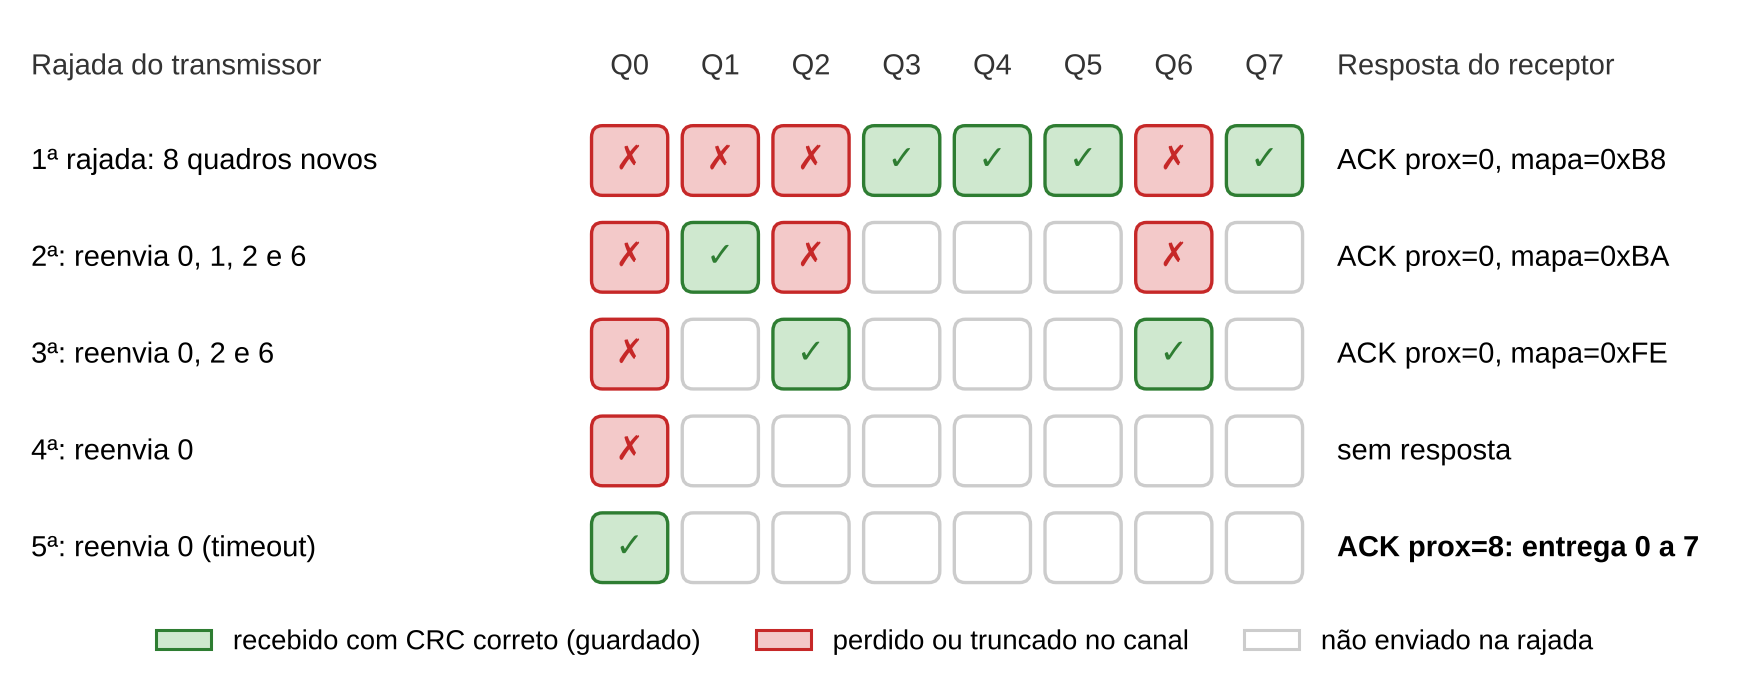
\includegraphics[width=15.5cm]{fig/matriz_sr.png}
  \fonte{Elaborado pelos autores a partir dos \textit{logs} de 21/11/2026.}
\end{figure}

A análise dos \textit{logs} revelou ainda que o primeiro quadro de cada rajada foi confirmado em 72\% das transmissões (165 de 229), contra 93\% dos demais quadros (482 de 516), nos ensaios sem erro ou perda simulados. O transmissor inicia a rajada cerca de 10 ms após receber o ACK, instante em que o receptor da placa B acabou de transmitir essa confirmação e ainda opera com ganho reduzido. Trata-se do mesmo efeito observado na placa A, agora no sentido oposto.

\section{Transmissão de imagem}

\begin{table}[H]
  \centering
  \caption{Resultados da transmissão de imagem (PNG de 490 bytes, 1 m)}
  \small\renewcommand{\arraystretch}{1.3}
  \begin{tabular}{|>{\raggedright\arraybackslash}m{3.09cm}|>{\centering\arraybackslash}m{2.06cm}|>{\centering\arraybackslash}m{2.41cm}|>{\centering\arraybackslash}m{2.92cm}|>{\centering\arraybackslash}m{3.27cm}|}
  \hline
  \rowcolor{gray!22}\textbf{Cenário} & \textbf{Entregues} & \textbf{Tempo médio} & \textbf{Retransmissões} & \textbf{SHA-256 igual ao original} \\ \hline
  Sem erro simulado & 3 de 3 & 44,1 s & 15,3 & 3 de 3 \\ \hline
  Com /erro 30 & 3 de 3 & 59,5 s & 32 & 3 de 3 \\ \hline
  \end{tabular}
  \fonte{Elaborado pelos autores a partir dos \textit{logs} de 21/11/2026.}
\end{table}

As seis imagens recebidas apresentaram o mesmo resumo SHA-256 do arquivo original. Em um arquivo binário, a inversão de um único bit já alteraria a imagem ou o resumo; a coincidência, portanto, comprova a integridade da transferência. A Figura 9 compara a imagem original com uma das recebidas.

\begin{figure}[H]
  \centering
  \caption{Imagem original e imagem reconstruída no computador receptor}
  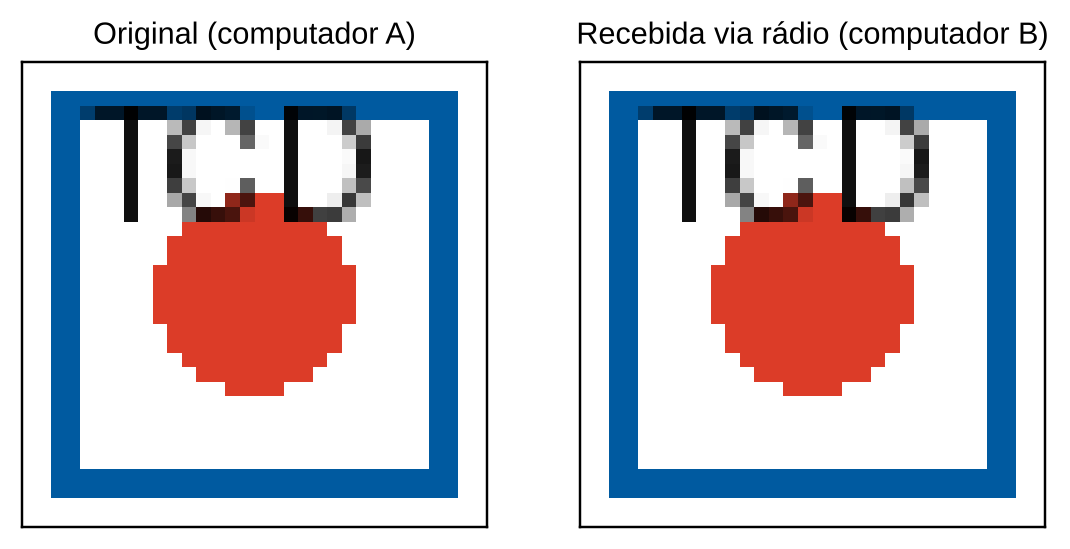
\includegraphics[width=10.0cm]{fig/imagem_comparacao.png}
  \fonte{Elaborado pelos autores (2026).}
\end{figure}

\section{Ensaios com dois computadores}

Em 23/11/2026, o enlace foi ensaiado na configuração prevista no enunciado, com cada placa ligada a um notebook diferente, conforme a Figura 10. A Tabela 18 apresenta os 21 ensaios de distância e de janela, realizados com o mesmo procedimento da campanha de 21/11.

\begin{figure}[H]
  \centering
  \caption{Placa A e notebook transmissor em primeiro plano; placa B e notebook receptor ao fundo}
  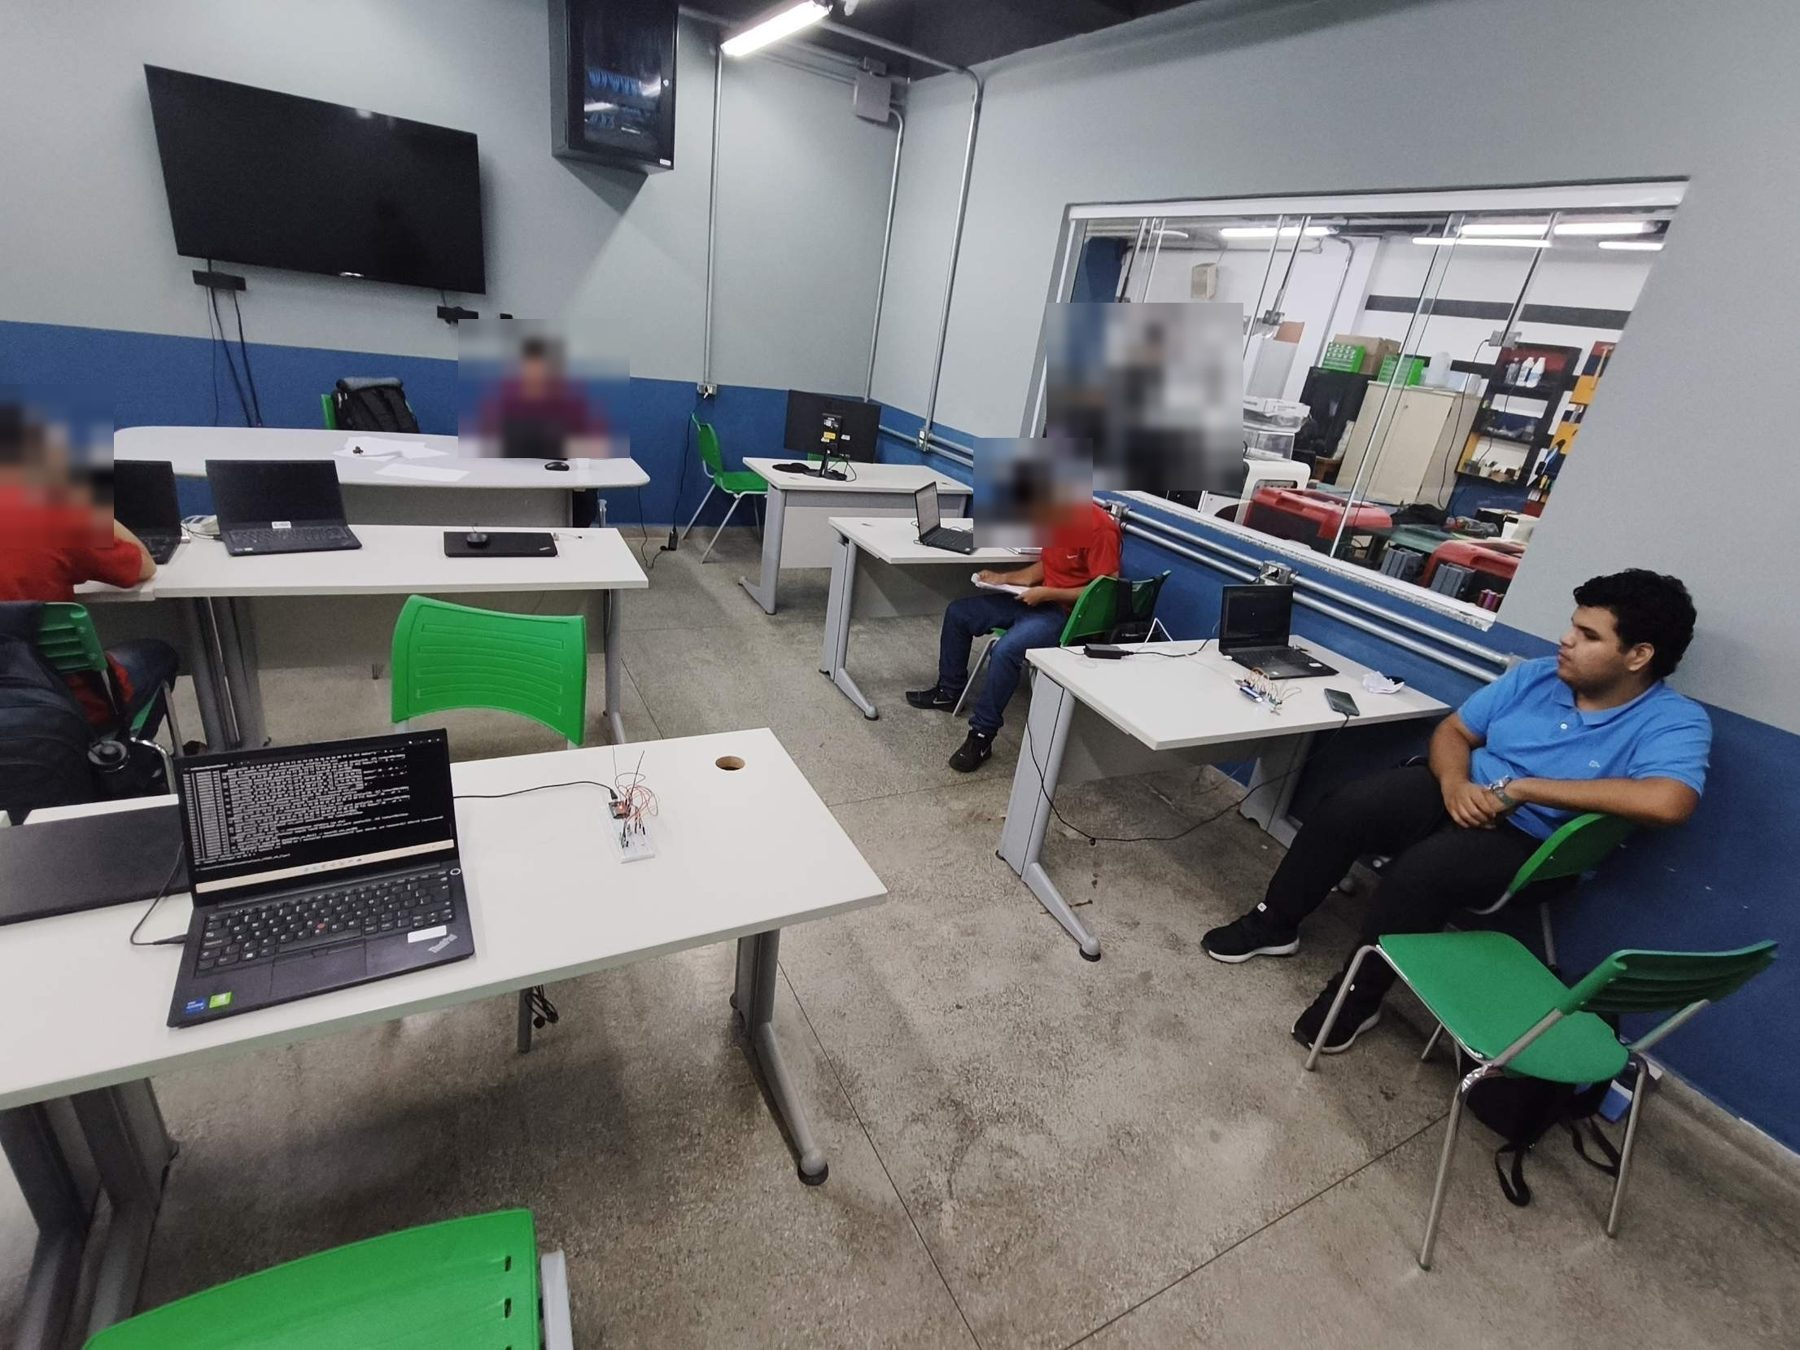
\includegraphics[width=13.0cm]{fig/dois_computadores.jpg}
  \fonte{Elaborado pelos autores (2026).}
\end{figure}

\begin{table}[H]
  \centering
  \caption{Resultados com uma placa em cada computador (mensagem de 201 bytes)}
  \small\renewcommand{\arraystretch}{1.3}
  \begin{tabular}{|>{\raggedright\arraybackslash}m{3.44cm}|>{\centering\arraybackslash}m{1.89cm}|>{\centering\arraybackslash}m{2.06cm}|>{\centering\arraybackslash}m{2.84cm}|>{\centering\arraybackslash}m{3.52cm}|}
  \hline
  \rowcolor{gray!22}\textbf{Cenário} & \textbf{Entregues} & \textbf{Tempo médio} & \textbf{Retransmissões} & \textbf{ACKs perdidos no retorno} \\ \hline
  0,5 m, janela 4 & 3 de 3 & 10,3 s & 0 & 0 \\ \hline
  1,0 m, janela 4 & 3 de 3 & 19,5 s & 6,7 & 0 \\ \hline
  1,5 m, janela 4 & 3 de 3 & 18,8 s & 6,0 & 0 \\ \hline
  2,0 m, janela 4 & 1 de 3 & 33,7 s & 17 & 0 na entrega; falhas sem recepção \\ \hline
  1 m, janela 1 (Stop-and-Wait) & 3 de 3 & 38,9 s & 13,3 & 1 \\ \hline
  1 m, janela 4 & 3 de 3 & 19,8 s & 7,3 & 1 \\ \hline
  1 m, janela 8 & 3 de 3 & 12,7 s & 3,0 & 0 \\ \hline
  \end{tabular}
  \fonte{Elaborado pelos autores a partir dos \textit{logs} de 23/11/2026.}
\end{table}

Das 21 mensagens, 19 foram entregues e todas chegaram idênticas às enviadas. O enlace manteve-se estável até 1,5 m. A 2 m, apenas uma mensagem foi entregue; nas duas falhas, o receptor não registrou nenhum quadro da mensagem e o transmissor abandonou-a após 20 s sem confirmação, o que situa o limite de alcance dessa disposição entre 1,5 m e 2 m. Diferentemente da campanha de 21/11, em que cerca de metade dos ACKs se perdia a 1 m e a 1,5 m, apenas dois ACKs deixaram de chegar ao transmissor em toda a bateria, o que indica que parte daquelas perdas estava associada à disposição das placas junto ao mesmo computador.

Com janela 8, a entrega foi 67\% mais rápida que com \textit{Stop-and-Wait}, contra 56\% em 21/11. A regularidade das retransmissões confirma a perda do primeiro quadro de cada rajada descrita na Seção 4.5: com janela 4, as mensagens de quatro rajadas exigiram em geral seis retransmissões; no \textit{Stop-and-Wait}, em que todo quadro é o primeiro da sua rajada, cerca de 13 dos 14 quadros precisaram ser retransmitidos por estouro do temporizador, o que praticamente dobrou o tempo de 18,3 s previsto pela Equação 6 para canal limpo.

Foram transmitidas duas imagens a 1,8 m: o mesmo PNG de 490 bytes da campanha de 21/11 e um PNG de 1280 × 1280 pixels com 2866 bytes, que ocupa 180 quadros DATA e um END. A Tabela 19 resume as duas transferências. Os contadores do receptor são acumulados desde a inicialização da placa; os valores da imagem de 2866 bytes foram obtidos pela diferença entre as estatísticas impressas ao final de cada imagem.

\begin{table}[H]
  \centering
  \caption{Transferência de imagens com dois computadores (1,8 m, janela 4)}
  \small\renewcommand{\arraystretch}{1.3}
  \begin{tabular}{|>{\raggedright\arraybackslash}m{6.57cm}|>{\centering\arraybackslash}m{4.04cm}|>{\centering\arraybackslash}m{4.04cm}|}
  \hline
  \rowcolor{gray!22}\textbf{Medida} & \textbf{PNG de 490 bytes} & \textbf{PNG de 2866 bytes} \\ \hline
  Quadros DATA + END & 31 + 1 & 180 + 1 \\ \hline
  Tempo de entrega no receptor & 64,5 s & 263,1 s \\ \hline
  Vazão útil & 7,6 bytes/s & 10,9 bytes/s \\ \hline
  Retransmissões (por ACK / por \textit{timeout}) & 31 (10 / 21) & – \\ \hline
  Quadros guardados fora de ordem & – & 135 \\ \hline
  Quadros truncados descartados & – & 6 \\ \hline
  Quadros rejeitados pelo CRC (erro real do canal) & 0 & 1 \\ \hline
  ACKs enviados pelo receptor & – & 94 \\ \hline
  SHA-256 igual ao original & sim & sim \\ \hline
  \end{tabular}
  \fonte{Elaborado pelos autores a partir dos \textit{logs} de 23/11/2026.}
\end{table}

Nos dois casos, o resumo SHA-256 calculado pelo enviar\_imagem.py antes da transmissão coincidiu com o calculado pelo receber\_imagem.py após a reconstrução, como mostra a Figura 11. Na transferência maior, o CRC rejeitou um quadro corrompido pelo próprio canal, sem erro simulado, e o quadro foi recuperado por retransmissão seletiva. O elevado número de quadros guardados fora de ordem decorre da perda do primeiro quadro de cada rajada, descrita na Seção 4.5: o receptor armazena os demais e aguarda apenas a retransmissão do ausente.

\begin{figure}[H]
  \centering
  \caption{SHA-256 da imagem de 2866 bytes no transmissor (a) e imagem reconstruída no receptor com o mesmo resumo (b)}
  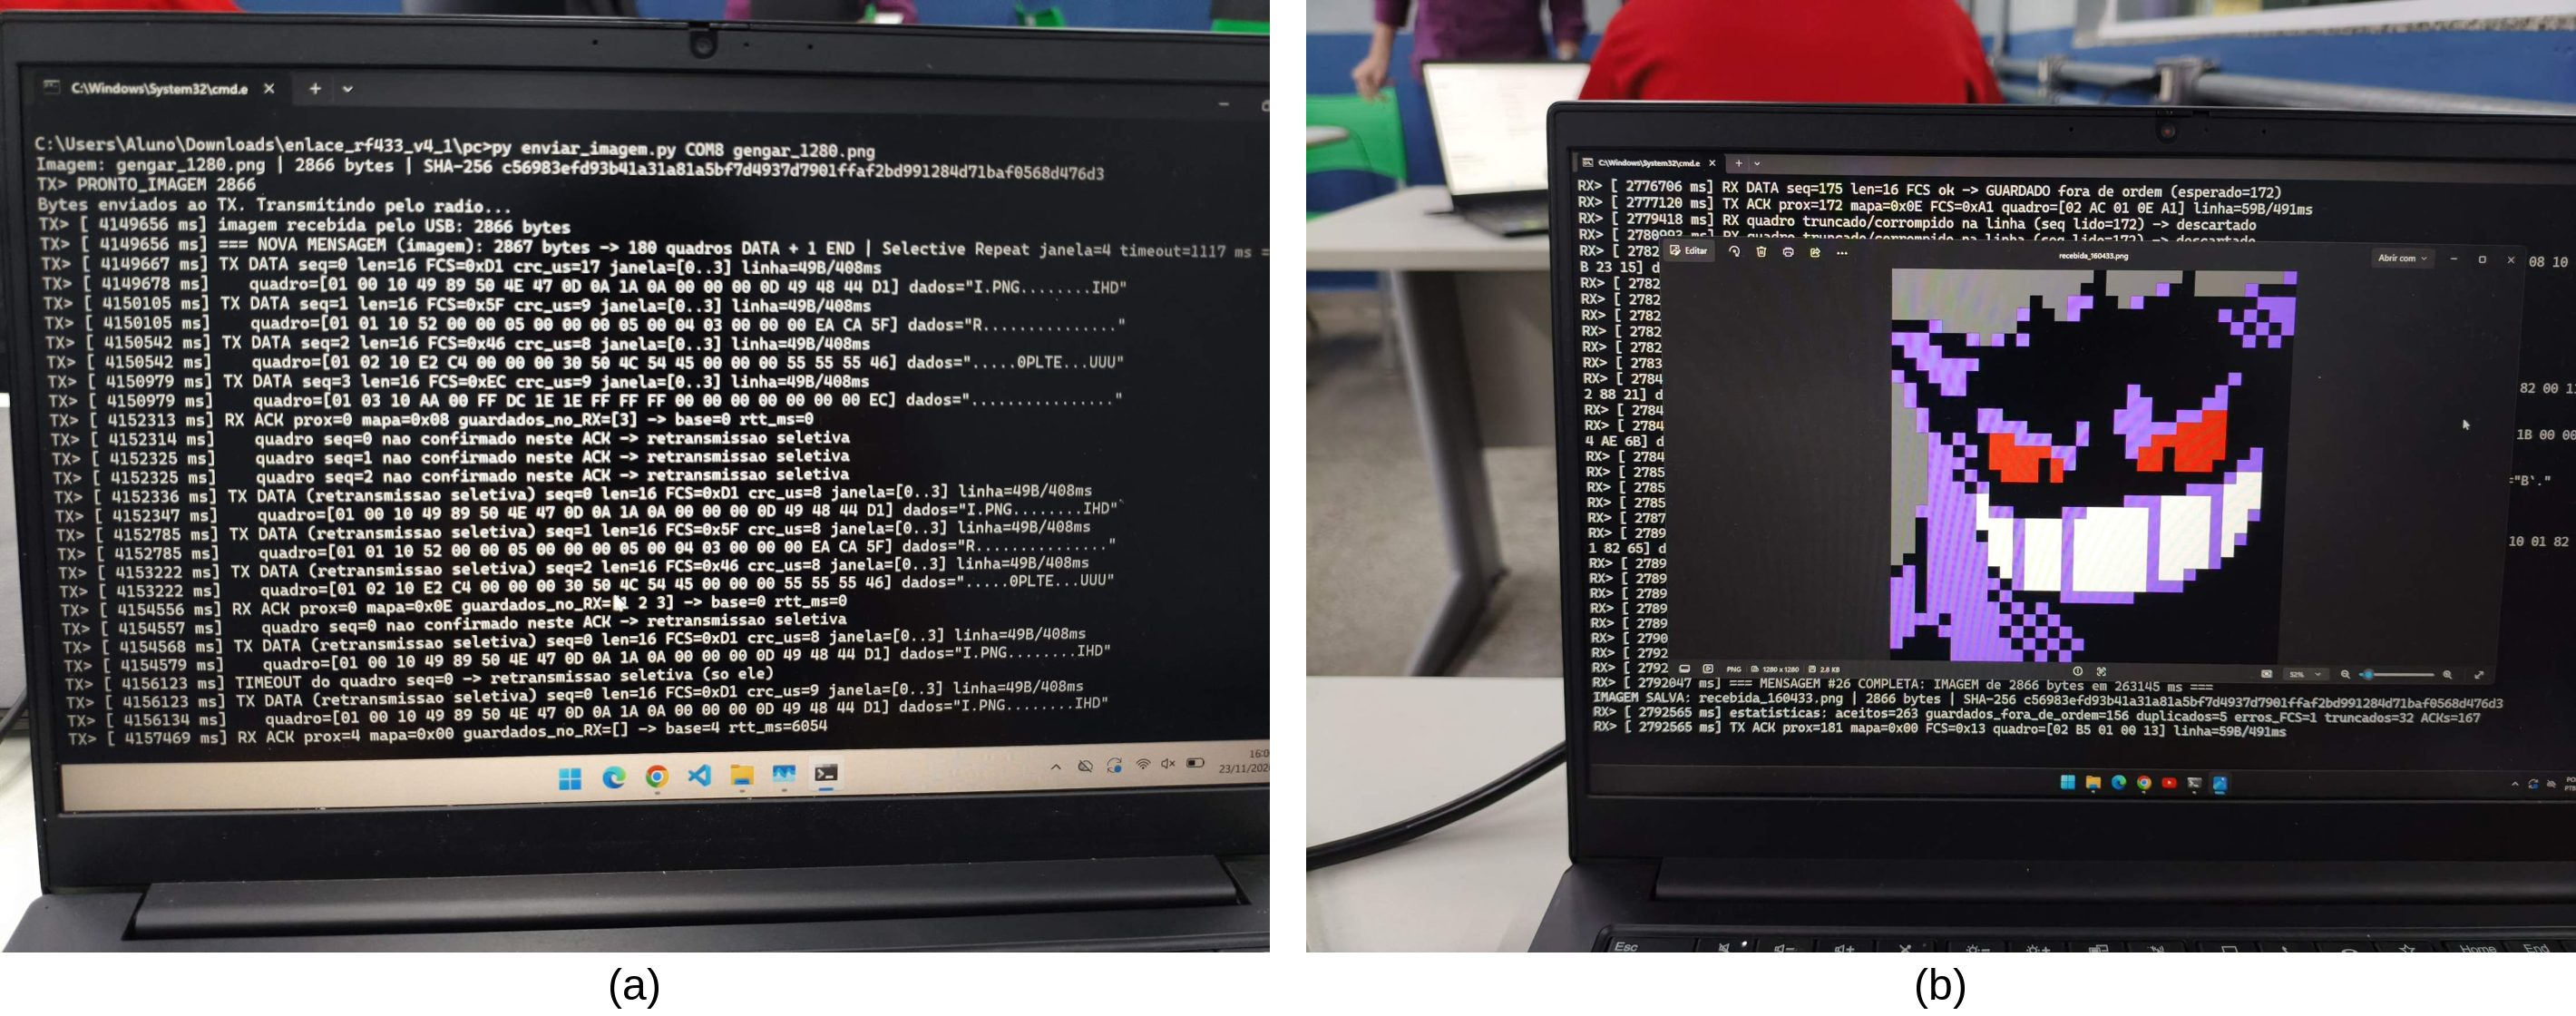
\includegraphics[width=15.5cm]{fig/gengar_tx_rx.jpg}
  \fonte{Elaborado pelos autores (2026).}
\end{figure}

A vazão útil de 10,9 bytes/s equivale a 87 bit/s, cerca de 7\% da taxa de 1200 bit/s da UART. A diferença corresponde à codificação Manchester, que dobra o número de bits, ao preâmbulo e ao cabeçalho de cada quadro, às esperas pelos ACKs e às retransmissões provocadas pela distância próxima do limite. O LCD da placa B exibiu tanto os textos recebidos quanto o aviso de chegada de cada imagem, conforme a Figura 12.

\begin{figure}[H]
  \centering
  \caption{LCD da placa B com texto recebido (a) e aviso de imagem de 2866 bytes (b)}
  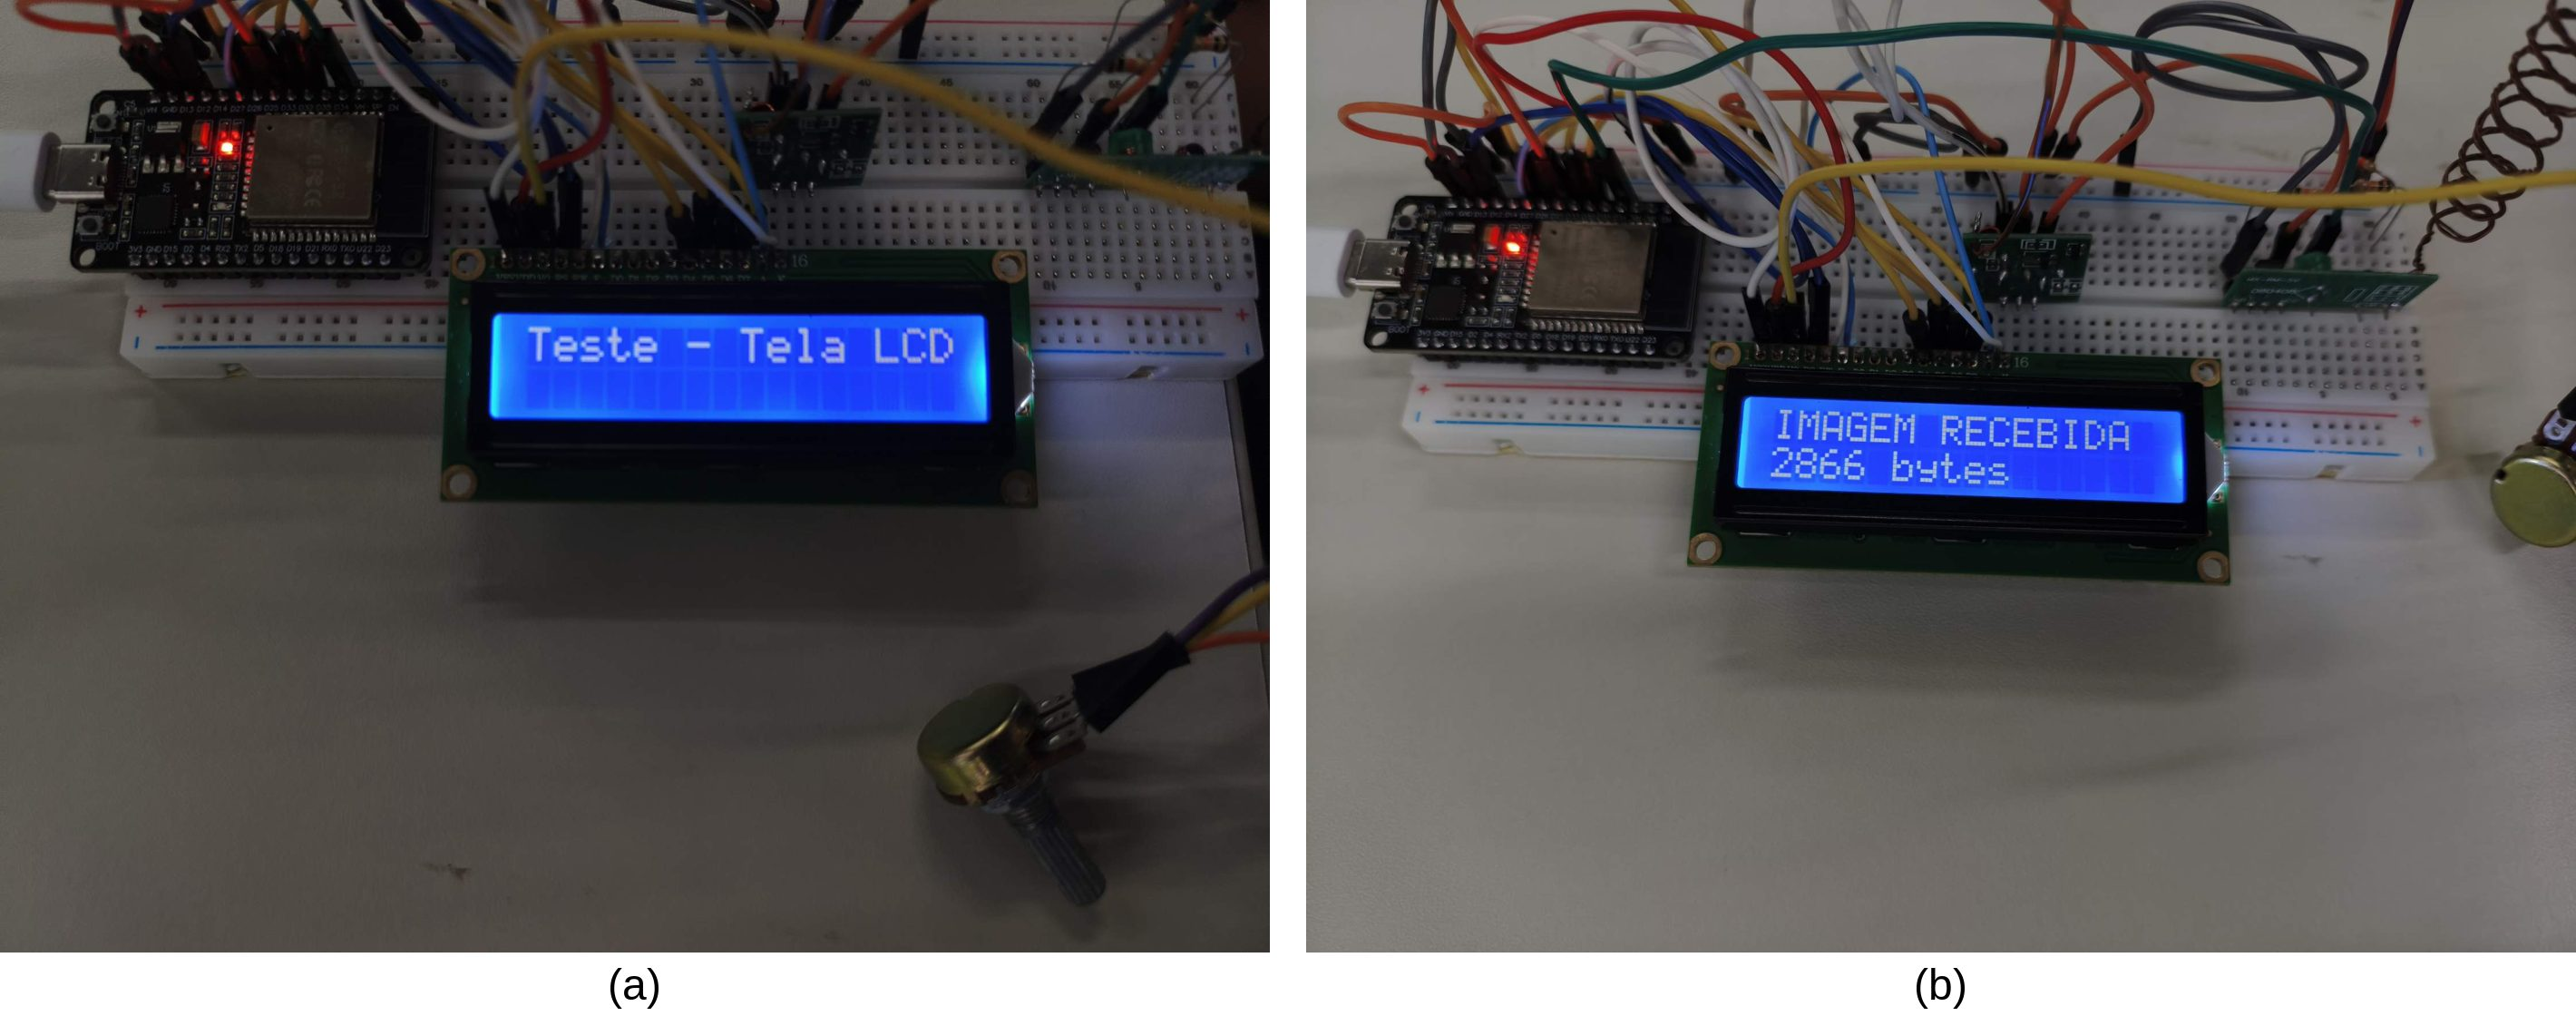
\includegraphics[width=15.5cm]{fig/lcd_texto_imagem.jpg}
  \fonte{Elaborado pelos autores (2026).}
\end{figure}

O comando /resumo, executado no transmissor ao final da sessão de cerca de 78 minutos, que incluiu as tentativas de alcance acima de 1,7 m, registrou 63 mensagens, 50 entregues e 13 abandonadas, com 896 quadros enviados e 566 retransmissões. Dessas, 495 ocorreram por estouro do temporizador e 71 por lacuna no mapa de bits do ACK. A predominância do \textit{timeout} confirma que, na distância limite, a perda concentra-se nas confirmações que retornam à placa A.

\section{Problemas encontrados durante o desenvolvimento}

A Tabela 20 registra os principais problemas encontrados ao longo do desenvolvimento, suas causas e as soluções adotadas. Os problemas concentraram-se na camada física, e não na lógica do protocolo.

\begin{table}[H]
  \centering
  \caption{Problemas encontrados e soluções adotadas}
  \small\renewcommand{\arraystretch}{1.3}
  \begin{tabular}{|>{\raggedright\arraybackslash}m{4.21cm}|>{\centering\arraybackslash}m{5.31cm}|>{\centering\arraybackslash}m{5.13cm}|}
  \hline
  \rowcolor{gray!22}\textbf{Problema} & \textbf{Causa} & \textbf{Solução} \\ \hline
  ACK nunca chegava ao transmissor & Nível 1 de repouso da UART mantinha o FS1000A transmitindo & UART com sinal invertido \\ \hline
  Alcance de 70 a 80 cm & Deformação dos pulsos a 2400 bit/s & Taxa de 1200 bit/s \\ \hline
  Dados chegavam e o ACK não & Receptor da placa A com ganho reduzido após transmitir & Silêncio de 300 ms antes do ACK e preâmbulo de 48 bytes \\ \hline
  Falhas intermitentes com uma placa no desktop & Ruído da fonte e das portas USB próximo ao receptor & Alimentação por notebook com bateria e placas afastadas \\ \hline
  Ruído interpretado como início de quadro & Saída aleatória do receptor ocioso & Manchester e limite LEN ≤ 16 \\ \hline
  Saída do receptor em 5 V & Alimentação de 5 V exigida pelo MX-RM-5V & Divisor de tensão para 3,3 V \\ \hline
  \end{tabular}
  \fonte{Elaborado pelos autores (2026).}
\end{table}

\section{Atendimento aos critérios do enunciado}

A Tabela 21 relaciona os requisitos e critérios de aceitação do enunciado às seções deste relatório que demonstram o seu atendimento.

\begin{table}[H]
  \centering
  \caption{Atendimento aos requisitos e critérios do enunciado}
  \small\renewcommand{\arraystretch}{1.3}
  \begin{tabular}{|>{\raggedright\arraybackslash}m{5.49cm}|>{\centering\arraybackslash}m{6.41cm}|>{\centering\arraybackslash}m{2.75cm}|}
  \hline
  \rowcolor{gray!22}\textbf{Requisito} & \textbf{Atendimento} & \textbf{Seção} \\ \hline
  Transmissão RF sem RadioHead & Camada física própria & 3.5 \\ \hline
  Quadro FLAG, TYPE, SEQ, LEN, DATA, FCS & Implementado conforme o enunciado & 3.3 \\ \hline
  Detecção de erros por CRC & CRC-8, 57 detecções, 0 aceites com erro & 3.4 e 4.4 \\ \hline
  Controle de erros por Selective Repeat & Janela de até 8 e ACK com mapa de bits & 3.6 e 4.5 \\ \hline
  Texto no LCD do receptor & LCD 16x2 com paginação & 3.7 e 4.7 \\ \hline
  Imagem reconstruída no laptop receptor & 8 de 8 imagens íntegras, 2 com dois computadores & 4.6 e 4.7 \\ \hline
  Distância superior a 1 m & Entregas até 2 m; estável até 1,5 m com dois computadores & 4.1 e 4.7 \\ \hline
  Funcionamento com ruído & 2 de 3 entregas íntegras com interferência & 4.3 \\ \hline
  Comunicação apenas por rádio & Sem condutor de dados entre as placas & 3.8 e 4.7 \\ \hline
  Dado em perfeito estado & 54 de 54 entregas sem erro & 4.1 a 4.7 \\ \hline
  \end{tabular}
  \fonte{Elaborado pelos autores (2026).}
\end{table}


\chapter{CONSIDERAÇÕES FINAIS}
O enlace implementado atendeu aos critérios de aceitação do enunciado. A comunicação ocorreu exclusivamente por rádio, alcançou 2 m, manteve-se operante sob interferência real e entregou 33 mensagens sem nenhum erro, incluindo seis imagens idênticas à original. Com uma placa em cada computador, uma imagem de 2866 bytes foi transferida a 1,8 m com resumo SHA-256 idêntico ao do arquivo enviado, e a repetição dos ensaios nessa configuração entregou 19 de 21 mensagens sem erro. Nos três casos em que o canal se degradou além do recuperável, o protocolo abandonou a mensagem em vez de entregar dado corrompido.

O CRC-8 rejeitou todos os quadros corrompidos que chegaram ao receptor, a um custo de cerca de 8 µs por quadro, e a codificação Manchester eliminou a maior parte dos erros reais do canal antes da verificação. O \textit{Selective Repeat} com janela 8 reduziu o tempo de entrega em 56\% em relação ao \textit{Stop-and-Wait}, ao distribuir a espera pela confirmação entre vários quadros e retransmitir somente os quadros perdidos.

A principal dificuldade residiu na camada física: módulos de baixo custo, canal \textit{half-duplex} e receptores sensíveis ao próprio transmissor e ao ruído da alimentação. Entre as limitações, destacam-se a vazão útil de cerca de 20 bytes/s no melhor caso, consequência da prioridade dada ao alcance, e o número reduzido de repetições por cenário, suficiente para caracterizar o comportamento, mas não para estimar taxas com precisão estatística.

Como trabalhos futuros, propõem-se a inserção de um intervalo de cerca de 300 ms após cada ACK antes da rajada seguinte, para mitigar a perda do primeiro quadro identificada na Seção 4.5, a alimentação do transmissor com tensão superior a 5 V, admitida pelo FS1000A, e a repetição dos ensaios com maior número de amostras em cada distância.


\postextual

\begin{thebibliography}{99}
\bibitem{r0} COOK, Greg. \textit{Catalogue of parametrised CRC algorithms}: CRC-8/SMBUS. [S. l.], 2026. Disponível em: \url{https://reveng.sourceforge.io/crc-catalogue/1-15.htm}. Acesso em: 21 nov. 2026.
\bibitem{r1} ESPRESSIF SYSTEMS. \textit{Arduino-ESP32}: Serial (UART). Shanghai: Espressif Systems, 2026. Disponível em: \url{https://docs.espressif.com/projects/arduino-esp32/en/latest/api/serial.html}. Acesso em: 21 nov. 2026.
\bibitem{r2} FOROUZAN, Behrouz A. \textit{Comunicação de dados e redes de computadores}. 4. ed. Porto Alegre: AMGH, 2010.
\bibitem{r3} INSTITUTO FEDERAL DE EDUCAÇÃO, CIÊNCIA E TECNOLOGIA DE MATO GROSSO (IFMT). \textit{Projeto final da disciplina Transmissão e Comunicação de Dados}: transmissão de dados confiável via rádio. Cuiabá: IFMT, 2026. Enunciado de projeto.
\bibitem{r4} OLIVEIRA, Ruy de. \textit{Transmissão e comunicação de dados}: notas de aula. Cuiabá: IFMT, 2026. Material de aula.
\bibitem{r5} TANENBAUM, Andrew S.; WETHERALL, David. \textit{Redes de computadores}. 5. ed. São Paulo: Pearson, 2011.
\end{thebibliography}

\begin{apendicesenv}
\chapter{Trechos do código-fonte}
Os trechos a seguir foram extraídos do \textit{firmware} final (versão 4.1), com a remoção dos comandos de registro no Monitor Serial, de contadores estatísticos e de tratamentos secundários, como a temporização entre bytes e a confirmação do quadro END. Os arquivos completos estão nos diretórios firmware/tx e firmware/rx do repositório; o arquivo protocolo\_rf.h é idêntico nas duas placas.

\section{Cálculo e verificação do CRC-8}

A função crc8 executa a divisão polinomial bit a bit pelo gerador 0x07, conforme a Seção 3.4. O FCS abrange os campos TYPE, SEQ, LEN e DATA; o receptor recalcula o valor sobre os campos recebidos e descarta o quadro quando o resultado difere do FCS transmitido.

\begin{Verbatim}[fontsize=\scriptsize,frame=single,framesep=2mm,rulecolor=\color{gray!60},breaklines,breakanywhere]
// protocolo_rf.h -- CRC-8: polinomio x^8 + x^2 + x + 1 (0x07), valor inicial 0x00,
// sem reflexao e sem XOR final (CRC-8/SMBUS).
inline uint8_t crc8(const uint8_t *p, size_t n) {
  uint8_t crc = 0x00;
  for (size_t i = 0; i < n; ++i) {
    crc ^= p[i];                         // soma o proximo byte ao registrador
    for (uint8_t b = 0; b < 8; ++b)      // divisao polinomial bit a bit
      crc = (crc & 0x80) ? uint8_t((crc << 1) ^ 0x07) : uint8_t(crc << 1);
  }
  return crc;
}

// FCS calculado sobre TYPE, SEQ, LEN e DATA (exclui FLAG e o proprio FCS).
inline uint8_t calculaFcs(const Quadro &q) {
  uint8_t buf[3 + MAX_DADOS];
  buf[0] = q.tipo; buf[1] = q.seq; buf[2] = q.len;
  for (uint8_t i = 0; i < q.len; ++i) buf[3 + i] = q.dados[i];
  return crc8(buf, 3 + q.len);
}

// Verificacao no receptor (dentro de Receptor::recebe, com o quadro completo):
fcsCalculado = calculaFcs(quadro);
if (fcsCalculado != quadro.fcs) return ERRO_FCS;      // quadro descartado
return QUADRO_OK;
\end{Verbatim}

\section{Montagem e desmontagem do quadro}

A função montaLinha produz a sequência enviada à UART2: preâmbulo, FLAG e os campos do quadro, com cada nibble convertido em um byte Manchester. No receptor, o método recebe processa um byte por vez, reconstrói os campos após a FLAG, rejeita bytes fora do código Manchester e valores de LEN acima de 16, e confere o FCS ao completar o quadro.

\begin{Verbatim}[fontsize=\scriptsize,frame=single,framesep=2mm,rulecolor=\color{gray!60},breaklines,breakanywhere]
// protocolo_rf.h -- campos do quadro e montagem dos bytes enviados pela UART2
constexpr uint8_t FLAG = 0x7E, PREAMBULO_BYTE = 0xF0, MAX_DADOS = 16;
enum Tipo : uint8_t { DATA = 0x01, ACK = 0x02, END = 0x03 };

struct Quadro {
  uint8_t tipo, seq, len;          // TYPE, SEQ, LEN
  uint8_t dados[MAX_DADOS];        // DATA (0 a 16 bytes)
  uint8_t fcs;                     // FCS = CRC-8
};

// Manchester por nibble: cada bit vira um par (1 -> "10", 0 -> "01").
inline uint8_t codificaNibble(uint8_t n) {
  uint8_t saida = 0;
  for (uint8_t i = 0; i < 4; ++i)
    saida |= uint8_t((((n >> i) & 1) ? 0b01 : 0b10) << (2 * i));
  return saida;
}

// Linha = preambulo + FLAG + (TYPE SEQ LEN DATA FCS) em Manchester.
inline size_t montaLinha(const Quadro &q, uint8_t *saida) {
  size_t n = 0;
  const uint8_t pre = (q.tipo == ACK) ? PREAMBULO_ACK_QTD : PREAMBULO_QTD;  // 48 ou 8
  for (uint8_t i = 0; i < pre; ++i) saida[n++] = PREAMBULO_BYTE;
  saida[n++] = FLAG;
  uint8_t campos[3 + MAX_DADOS + 1], total = 0;
  campos[total++] = q.tipo; campos[total++] = q.seq; campos[total++] = q.len;
  for (uint8_t i = 0; i < q.len; ++i) campos[total++] = q.dados[i];
  campos[total++] = q.fcs;
  for (uint8_t i = 0; i < total; ++i) {
    saida[n++] = codificaNibble(campos[i] >> 4);     // nibble alto primeiro
    saida[n++] = codificaNibble(campos[i] & 0x0F);
  }
  return n;
}

// Desmontagem (resumida): Receptor::recebe(byte) e chamado a cada byte da UART2.
Resultado recebe(uint8_t b, uint32_t agoraMs) {
  if (buscando_) { if (b == FLAG) comecaQuadro(agoraMs); return NADA; }
  const int8_t nib = decodificaNibble(b);          // -1 se o byte nao e Manchester
  if (nib < 0) return abandona();                  // quadro truncado ou ruido
  if (nibbleAlto_ < 0) { nibbleAlto_ = nib; return NADA; }
  bruto_[n_++] = uint8_t((nibbleAlto_ << 4) | nib);
  nibbleAlto_ = -1;
  if (n_ == 3 && bruto_[2] > MAX_DADOS) return abandona();   // LEN impossivel
  if (n_ < 3u + bruto_[2] + 1u) return NADA;                 // faltam bytes
  buscando_ = true;                                          // quadro completo
  quadro.tipo = bruto_[0]; quadro.seq = bruto_[1]; quadro.len = bruto_[2];
  memcpy(quadro.dados, bruto_ + 3, quadro.len);
  quadro.fcs = bruto_[3 + quadro.len];
  fcsCalculado = calculaFcs(quadro);
  return fcsCalculado == quadro.fcs ? QUADRO_OK : ERRO_FCS;
}
\end{Verbatim}

\section{Janela deslizante do Selective Repeat}

No transmissor, executaSelectiveRepeat prioriza a retransmissão de quadros pendentes, envia quadros novos enquanto houver espaço na janela e arma um temporizador por quadro ao final da rajada. O método trataAck confirma de forma cumulativa os quadros anteriores a SEQ, confirma individualmente os indicados no mapa de bits e marca para reenvio apenas os quadros ausentes.

\begin{Verbatim}[fontsize=\scriptsize,frame=single,framesep=2mm,rulecolor=\color{gray!60},breaklines,breakanywhere]
// tx.ino -- Selective Repeat no transmissor (chamado a cada volta do loop)
void executaSelectiveRepeat() {
  if (!ativo) return;
  if (base == totalQuadros) { finalizaMensagem(true); return; }
  const uint32_t agora = millis();

  // 1) Retransmissao seletiva: quadro apontado pelo ACK ou com timeout.
  for (uint32_t i = base; i < proximo; ++i) {
    if (confirmado[i] || prazo[i] == 0) continue;
    if (prazo[i] == REENVIAR_JA || int32_t(agora - prazo[i]) >= 0) {
      enviaQuadro(i);
      return;
    }
  }
  // 2) Quadro novo, se couber na janela; o END so sai com todos os DATA confirmados.
  const bool ehEnd = (proximo == quadrosDados);
  const bool cabe = proximo < base + janela;
  if (proximo < totalQuadros && cabe && (!ehEnd || base == quadrosDados)) {
    enviaQuadro(proximo++);
    return;
  }
  // 3) Fim da rajada: arma um temporizador por quadro pendente e aguarda o ACK.
  for (uint32_t i = base; i < proximo; ++i)
    if (!confirmado[i] && prazo[i] == 0) prazo[i] = agora + TIMEOUT_ACK_MS; // 1117 ms
  if (agora - ultimoProgressoMs > DESISTENCIA_TX_MS) finalizaMensagem(false);  // 20 s
}

// ACK seletivo: SEQ = proximo quadro esperado em ordem;
// bit b do mapa = quadro SEQ + b ja guardado pelo receptor.
void trataAck(uint8_t seq, uint8_t mapa) {
  int32_t k = -1;                        // indice absoluto correspondente a SEQ
  for (uint32_t i = base; i <= proximo && i <= base + JANELA_MAX; ++i)
    if (uint8_t(i & 0xFF) == seq) { k = int32_t(i); break; }
  if (k < 0) return;                                // ACK fora da janela: ignorado

  for (uint32_t i = base; i < uint32_t(k); ++i) confirmado[i] = true;  // cumulativo
  for (uint8_t b = 0; b < 8; ++b) {                           // mapa de bits
    const uint32_t i = uint32_t(k) + b;
    if (((mapa >> b) & 1) && i < proximo) confirmado[i] = true;
  }
  while (base < totalQuadros && confirmado[base]) ++base;     // desliza a janela

  // Quadro enviado antes deste ACK e nao confirmado foi perdido: reenvia so ele.
  for (uint32_t i = base; i < proximo; ++i)
    if (!confirmado[i] && jaEnviado[i] &&
        enviadoMs[i] + ESPERA_ANTES_ACK_MS + DURACAO_ACK_MS <= millis() + 10)
      prazo[i] = REENVIAR_JA;
}
\end{Verbatim}

No receptor, cada quadro DATA válido é armazenado na posição correspondente da janela, mesmo fora de ordem, e entregaEmOrdem repassa à mensagem a sequência contínua a partir do quadro esperado. Após o silêncio do canal, o receptor envia um único ACK com o próximo SEQ esperado e o mapa de bits dos quadros já guardados.

\begin{Verbatim}[fontsize=\scriptsize,frame=single,framesep=2mm,rulecolor=\color{gray!60},breaklines,breakanywhere]
// rx.ino -- trataQuadro(), ramo do DATA com FCS correto (janela de 8 quadros)
if (q.tipo == rf::DATA && q.len > 0) {
  ackPendente = true;
  const uint8_t d = uint8_t(q.seq - esperado);   // posicao na janela (mod 256)
  if (d < JANELA_RX) {
    if (guardado[d]) return;                     // duplicado: descarta
    guardado[d] = true;                          // guarda, mesmo fora de ordem
    lenGuardado[d] = q.len;
    memcpy(dadosGuardados[d], q.dados, q.len);
    temAck = true;
    entregaEmOrdem();
  }                                  // d >= 128: ja entregue; o ACK repete
}

// Entrega a mensagem enquanto houver sequencia continua a partir de 'esperado'.
void entregaEmOrdem() {
  while (guardado[0]) {
    memcpy(mensagem + tamanhoMensagem, dadosGuardados[0], lenGuardado[0]);
    tamanhoMensagem += lenGuardado[0];
    for (uint8_t i = 0; i + 1 < JANELA_RX; ++i) {   // desliza a janela
      guardado[i] = guardado[i + 1];
      lenGuardado[i] = lenGuardado[i + 1];
      memcpy(dadosGuardados[i], dadosGuardados[i + 1], MAX_DADOS);
    }
    guardado[JANELA_RX - 1] = false;
    ++esperado;                                     // uint8_t: 255 -> 0
  }
}

// Um ACK por rajada, apos 425 ms de silencio (ramo que confirma o END omitido).
void enviaAckSeNecessario() {
  if (!ackPendente || receptor.recebendo()) return;
  if (millis() - ultimaAtividadeMs < ESPERA_ANTES_ACK_MS) return;
  ackPendente = false;
  if (!temAck) return;                 // nada novo para confirmar
  rf::Quadro ack;
  ack.tipo = rf::ACK; ack.len = 1;
  ack.seq = esperado;                    // proximo esperado em ordem
  uint8_t mapa = 0;                      // bit i = quadro (esperado + i) guardado
  for (uint8_t i = 0; i < JANELA_RX; ++i) if (guardado[i]) mapa |= uint8_t(1 << i);
  ack.dados[0] = mapa;
  ack.fcs = rf::calculaFcs(ack);
  uint8_t linha[rf::MAX_LINHA];
  transmiteLinha(linha, rf::montaLinha(ack, linha));
}
\end{Verbatim}

\chapter{Trechos dos logs do Monitor Serial}
Os trechos a seguir foram extraídos dos \textit{logs} do Monitor Serial gravados durante a bateria de ensaios. Os arquivos completos dos 36 ensaios, um por placa e por ensaio, estão no diretório evidencias/2026-11-21\_1258/logs do repositório.

\section{Mensagem a 0,5 m sem retransmissões (transmissor)}

\begin{Verbatim}[fontsize=\scriptsize,frame=single,framesep=2mm,rulecolor=\color{gray!60},breaklines,breakanywhere]
=== NOVA MENSAGEM (texto): 201 bytes -> 13 quadros DATA + 1 END | Selective Repeat
    janela=4 timeout=1117 ms ===
TX DATA seq=0 len=16 FCS=0x42 crc_us=16 janela=[0..3] linha=49B/408ms
   quadro=[01 00 10 54 41 42 43 44 45 46 47 48 49 4A 4B 4C 4D 4E 4F 42]
...
RX ACK prox=4 mapa=0x00 guardados_no_RX=[] -> base=4 rtt_ms=899
RX ACK prox=8 mapa=0x00 guardados_no_RX=[] -> base=8 rtt_ms=899
RX ACK prox=12 mapa=0x00 guardados_no_RX=[] -> base=12 rtt_ms=899
...
=== MENSAGEM ENTREGUE em 10263 ms | envios=14 retransmissoes=0 (por ACK=0,
    por timeout=0) ACKs=5 (ignorados=0) erros_sim=0 perdas_sim=0 | 19.6 bytes/s ===
\end{Verbatim}

\section{Retransmissão seletiva com janela 8 (transmissor)}

\begin{Verbatim}[fontsize=\scriptsize,frame=single,framesep=2mm,rulecolor=\color{gray!60},breaklines,breakanywhere]
RX ACK prox=0 mapa=0xB8 guardados_no_RX=[3 4 5 7] -> base=0 rtt_ms=0
   quadro seq=0 nao confirmado neste ACK -> retransmissao seletiva
   quadro seq=1 nao confirmado neste ACK -> retransmissao seletiva
   quadro seq=2 nao confirmado neste ACK -> retransmissao seletiva
   quadro seq=6 nao confirmado neste ACK -> retransmissao seletiva
TX DATA (retransmissao seletiva) seq=0 len=16 FCS=0x42 crc_us=9 janela=[0..7]
\end{Verbatim}

\section{Detecção pelo CRC com /erro 30 (receptor)}

\begin{Verbatim}[fontsize=\scriptsize,frame=single,framesep=2mm,rulecolor=\color{gray!60},breaklines,breakanywhere]
RX DATA seq=5 len=16 FCS ok -> GUARDADO fora de ordem (esperado=4)
RX quadro DATA seq=6: FCS recebido=0x07 calculado=0x33 -> ERRO DETECTADO, descartado
RX DATA seq=7 len=16 FCS ok -> GUARDADO fora de ordem (esperado=4)
...
RX quadro DATA seq=4: FCS recebido=0xF0 calculado=0xBF -> ERRO DETECTADO, descartado
\end{Verbatim}

\section{Mensagem abandonada a 1 m (transmissor)}

\begin{Verbatim}[fontsize=\scriptsize,frame=single,framesep=2mm,rulecolor=\color{gray!60},breaklines,breakanywhere]
=== FALHA: MENSAGEM ABANDONADA em 25317 ms | envios=36 retransmissoes=24 (por ACK=0,
    por timeout=24) ACKs=2 (ignorados=0) erros_sim=0 perdas_sim=0 | 7.9 bytes/s ===
\end{Verbatim}

\end{apendicesenv}

\end{document}
